% cd /mnt/ExtraDrive1/Work/desktop_data/2022_papers/hglmm/Github/hglmm
% bibtex hglmm

\documentclass[12pt, titlepage]{article}

\usepackage{alltt}
\usepackage{graphicx, amsmath, amssymb, natbib, setspace}
\usepackage{float}
\usepackage{booktabs,array}
\usepackage[caption = false]{subfig}
\usepackage{cancel}

\usepackage{/mnt/ExtraDrive1/Work/shTex/mymacros}
\setlength{\parindent}{3em}
 
\usepackage{caption}
 
\pdfpagewidth 8.5in
\pdfpageheight 11in
\setlength{\oddsidemargin}{0.0in} \setlength{\textwidth}{6.5in}
\setlength{\topmargin}{0.15in} \setlength{\textheight}{8.5in}
\setlength{\headheight}{0.0in} \setlength{\headsep}{0.0in}

\usepackage{makecell}%To keep spacing of text in tables
\setcellgapes{5pt}%parameter for the spacing

%%%%%%%%%%%%%%%%%%%%%%%%%%%%%%%%%%%%%%%%%%%%%%%%%%%%%%%%%%%%%%%%%%%%%%%%%%%%%%%%
%%%%%%%%%%%%%%%%%%%%%%%%%%%%%%%%%%%%%%%%%%%%%%%%%%%%%%%%%%%%%%%%%%%%%%%%%%%%%%%%
%%%%%%%%%%%%%%%%%%%%%%%%%%%%%%%%%%%%%%%%%%%%%%%%%%%%%%%%%%%%%%%%%%%%%%%%%%%%%%%%
% TITLE
%%%%%%%%%%%%%%%%%%%%%%%%%%%%%%%%%%%%%%%%%%%%%%%%%%%%%%%%%%%%%%%%%%%%%%%%%%%%%%%%
%%%%%%%%%%%%%%%%%%%%%%%%%%%%%%%%%%%%%%%%%%%%%%%%%%%%%%%%%%%%%%%%%%%%%%%%%%%%%%%%
%%%%%%%%%%%%%%%%%%%%%%%%%%%%%%%%%%%%%%%%%%%%%%%%%%%%%%%%%%%%%%%%%%%%%%%%%%%%%%%%

\IfFileExists{upquote.sty}{\usepackage{upquote}}{}
\begin{document}
\singlespacing

\titlepage
\title {Marginal Inference for Hierarchical Generalized Linear Mixed Models with Patterned Covariance Matrices using the Laplace Approximation}
\author{Jay M. Ver Hoef$^{1}$, Eryn Blagg$^{2}$, Michael Dumelle$^{3}$, Philip Dixon$^{2}$,  \\
 Dale Zimmerman$^{4}$, Paul Conn$^{1}$ \\
\hrulefill \\ 
$^{1}$National Marine Mammal Laboratory \\
NOAA-NMFS Alaska Fisheries Science Center\\
7600 Sand Point Way NE, Seattle, WA 98115\\
E-mail: jay.verhoef@noaa.gov\\
\hrulefill \\
$^{2}$ Department of Statistics, Iowa State University, Ames, Iowa \\
$^{3}$ United States Environmental Protection Agency, \\
	200 SW 35th St, Corvallis, Oregon \\
$^{4}$ Department of Statistics and Actuarial Science, \\
	The University of Iowa, Iowa City, Iowa \\
\hrulefill \\
}

\maketitle


\doublespacing

%%%%%%%%%%%%%%%%%%%%%%%%%%%%%%%%%%%%%%%%%%%%%%%%%%%%%%%%%%%%%%%%%%%%%%%%%%%%%%%%
%%%%%%%%%%%%%%%%%%%%%%%%%%%%%%%%%%%%%%%%%%%%%%%%%%%%%%%%%%%%%%%%%%%%%%%%%%%%%%%%
%%%%%%%%%%%%%%%%%%%%%%%%%%%%%%%%%%%%%%%%%%%%%%%%%%%%%%%%%%%%%%%%%%%%%%%%%%%%%%%%
% ABSTRACT
%%%%%%%%%%%%%%%%%%%%%%%%%%%%%%%%%%%%%%%%%%%%%%%%%%%%%%%%%%%%%%%%%%%%%%%%%%%%%%%%
%%%%%%%%%%%%%%%%%%%%%%%%%%%%%%%%%%%%%%%%%%%%%%%%%%%%%%%%%%%%%%%%%%%%%%%%%%%%%%%%
%%%%%%%%%%%%%%%%%%%%%%%%%%%%%%%%%%%%%%%%%%%%%%%%%%%%%%%%%%%%%%%%%%%%%%%%%%%%%%%%

\begin{abstract}
We take a fully parametric approach to creating covariance dependence for generalized linear mixed models through a hierarchical construction. We estimate covariance parameters and fixed effects marginally while integrating out over all latent random effects using the Laplace approximation. We use Newton-Raphson updates, which also leads to predictions for latent random effects.  We provide complete marginal inference, from estimating covariance parameters and fixed effects, to making predictions for unobserved data, for any patterned covariance matrix in the hierarchical generalized linear mixed models framework. We show how the marginal likelihood can be developed for six commonly used distributions that are often used for binary, count, and positive continuous data.  The methods are illustrated with simulations from known parameters, and their efficacy is shown through simulation experiments.  Three examples are used to illustrate all six distributions with a variety of patterned covariance structures that include spatial models, time series models, and mixtures with typical random intercepts based on grouping.
\end{abstract}

%%%%%%%%%%%%%%%%%%%%%%%%%%%%%%%%%%%%%%%%%%%%%%%%%%%%%%%%%%%%%%%%%%%%%%%%%%%%%%%%
%%%%%%%%%%%%%%%%%%%%%%%%%%%%%%%%%%%%%%%%%%%%%%%%%%%%%%%%%%%%%%%%%%%%%%%%%%%%%%%%
%%%%%%%%%%%%%%%%%%%%%%%%%%%%%%%%%%%%%%%%%%%%%%%%%%%%%%%%%%%%%%%%%%%%%%%%%%%%%%%%
%       \section{INTRODUCTION}
%%%%%%%%%%%%%%%%%%%%%%%%%%%%%%%%%%%%%%%%%%%%%%%%%%%%%%%%%%%%%%%%%%%%%%%%%%%%%%%%
%%%%%%%%%%%%%%%%%%%%%%%%%%%%%%%%%%%%%%%%%%%%%%%%%%%%%%%%%%%%%%%%%%%%%%%%%%%%%%%%
%%%%%%%%%%%%%%%%%%%%%%%%%%%%%%%%%%%%%%%%%%%%%%%%%%%%%%%%%%%%%%%%%%%%%%%%%%%%%%%%

\newpage
\section{INTRODUCTION}

The classical linear model relies on a normal distribution that has continuous support on the real line, but many data are binary, counts, or positive continuous.  Such data can be transformed to stabilize variances and create empirical distributions that are ``near normal,'' allowing the use of classical linear models \citep[e.g.,][ p. 288]{SnedecorEtAl1980StatisticalMethodsSeventh}. For example, a square root transformation can be used for count data.  However, \citet{NelderEtAl1972GeneralizedLinearModels370} introduced the generalized linear model \citep[GLM,][]{McCullaghEtAl1989GeneralizedLinearModels} as a natural extension to linear models, such as the Poisson distribution for counts, the Bernoulli distribution for binary data, etc., which have become very popular and generally preferred to data transformations \citep[e.g.,][]{warton_arcsine_2011}.  GLMs can be extended by introducing latent random effects as a linear mixed model to create a class of generalized linear mixed models \citep[GLMM,][]{breslow_approximate_1993}.  These latent random effects are usually assumed to be independent and identically distributed from a normal distribution \citep{zeger_generalized_1991}, however it is also possible for the latent random effects to be temporally autocorrelated \citep[e.g.,][]{stiratelli_random-effects_1984, zeger_models_1988}, spatially autocorrelated \citep[e.g,][]{clayton_empirical_1987, GotwayEtAl1997GeneralizedLinearModel157, DiggleEtAl1998ModelbasedGeostatisticsDisc299}, or both \citep[][p. 380]{CressieEtAl2011StatisticsSpatiotemporalData}.  A unifying framework for this literature is through a hierarchical generalized linear mixed model \citep[HGLMM,][]{lee_hierarchical_1996}.

%%%%%%%%%%%%%%%%%%%%%%%%%%%%%%%%%%%%%%%%%%%%%%%%%%%%%%%%%%%%%%%%%%%%%%%%%%%%%%%%
%               Hierarchical Generalized Linear Mixed Models
%%%%%%%%%%%%%%%%%%%%%%%%%%%%%%%%%%%%%%%%%%%%%%%%%%%%%%%%%%%%%%%%%%%%%%%%%%%%%%%%

\subsection{Hierarchical Generalized Linear Mixed Models}

Most GLMs are motivated by the exponential family of distributions \citep[e.g.,][]{fisher_two_1934, lehmann_theory_2006}.  However, GLMs are ultimately modeled with quasi-likelihood through the first two moments, the variance and mean functions,  and fitted through iteratively-weighted least-squares estimation \citep{wedderburn_quasi-likelihood_1974}, which creates a very flexible class of models. In fact, some models have no true likelihood, such as the quasi-Poisson model.

We will take a fully parametric approach to create covariance dependence for GLMMs through a hierarchical construction.  We will use the notation $[\by|\bmu]$ to denote any probability density function of the vector of random variables $\by$ conditional on a vector of parameters, or other fixed variables, $\bmu$. We can have a joint distribution on the left side of the conditional bar, and multiple parameter and fixed value vectors on the right, e.g., $[\by_{1},\by_{2}, \ldots, \by_{k} | \bmu_{1}, \bmu_{2}, \ldots, \bmu_{\ell}]$. For example, let $[\by|\bmu]$ be the product of independent Poisson distributions with mean parameters contained in the vector $\bmu$, so $\textrm{E}(\by) = \bmu$. The model for the data $\by$ can have more parameters than just the mean, in which case we write it $[\by|\bmu,\bphi]$. For an example with extra parameters for $\by$, consider the product of independent negative binomial distributions, which can be parameterized with a mean vector, and a common extra parameter that allows for overdispersion, which we would write as $[\by|\bmu,\phi]$, where $\phi$ is the overdispersion parameter.

For the hierarchical construction of the generalized linear mixed models that we consider in this article, we allow the mean to vary by other random variables $\bw$, and we condition on these random variables, $[\by|g^{-1}(\bw),\bphi]$, through the mean function $\textrm{E}(\by) = g^{-1}(\mathbf{w})$. For the Poisson example, $g(\cdot)$ is often the log function, and in general $g(\cdot)$ is called the link function \citep{McCullaghEtAl1989GeneralizedLinearModels}.  Link functions are monotonic so that $g^{-1}(\cdot)$ is one-to-one with $g(\cdot)$. Recall that the mean of a Poisson distribution must be positive, and if $g(\cdot)$ is the log function, then $g^{-1}(\cdot)$ is the exponential function so $\bmu = g^{-1}(\bw)$ is always positive, which allows $\bw$ to be unconstrained on the real line.

We will only consider models where $\bw$ is $n \times 1$ and has a multivariate normal distribution which is constructed through the linear mixed model,
\begin{equation} \label{eq:lm_eta}
\bw = \bX\bbeta + \sum_{k=1}^{q}\bZ_{k}\br_{k} + \bepsilon,
\end{equation}
where $\bX$ is an $n \times p$ full rank design matrix of explanatory variables, $\bbeta$ is a $p \times 1$ parameter vector of fixed effects, $\bZ_{k}$ is a design matrix for the $k$th random effect $\br_{k}$, and $\bepsilon$ is independent error.  We assume that $\textrm{E}(\br_{k}) = \bzero$ for all $k$, $\textrm{E}(\bepsilon) = \bzero$, $\var(\br_{k}) = \bV_{k}$, $\cov(\br_{j}, \br_{k}) = \bzero$ when $j \ne k$, and $\var(\bepsilon) = \sigma^{2}_{0}\bI$. We use the notation $[\bw|\bX,\bbeta,\{\bZ_{k}\},\{\bV_{k}\},\btheta]$ to indicate the probability density function $\bw \sim N(\bX\bbeta,\bSigma_{\btheta})$ where 
$$
\bSigma_{\btheta} = \sum_{k}\bZ_{k}\bV_{k}\bZ_{k}\upp + \sigma^{2}_{0}\bI.
$$
The covariance matrices $\{\bV_{k}\}$ for $k = 1,\ldots,q$ can have additional covariance parameters beyond $\sigma^{2}_{0}$, all of which are contained in the vector $\btheta$.  We will give more specific details on $\bSigma_{\btheta}$ later.

For the fully parametric, hierarchical models, a very general model can be constructed hierarchically as,
\begin{equation} \label{eq:hglmm}
[\by,\bw|\bphi,\bX,\bbeta,\bSigma_{\btheta}] = [\by|g^{-1}(\bw),\bphi][\bw|\bX, \bbeta,\bSigma_{\btheta}],
\end{equation}
where \citet{berliner_hierarchical_1996} called $[\by|g^{-1}(\bw),\bphi]$ the \textit{data model} and $[\bw|\bX, \bbeta,\bSigma_{\btheta}]$ the \textit{process model}. As a concrete example, suppose that $[\by|\exp(\bw)]$ is Poisson, and $[\bw|\bX,\bbeta,\bSigma_{\btheta}]$ is multivariate normal, then the joint likelihood is
$$
[\by,\bw|\bX,\bbeta,\bSigma_{\btheta}] = \left(\prod_{i=1}^{n}\frac{\exp(w_{i})^{y_{i}}\exp(-\exp(w_i))}{y_{i}!}\right)\frac{\exp\left(-(\bw - \bX\bbeta)\upp\bSigma_{\btheta}^{-1}(\bw - \bX\bbeta)\right)}{(2\pi)^{n/2}|\bSigma_{\btheta}|^{1/2}},
$$
and note the use of $\exp(w_{i})$ for $\textrm{E}(y_{i})$.

%%%%%%%%%%%%%%%%%%%%%%%%%%%%%%%%%%%%%%%%%%%%%%%%%%%%%%%%%%%%%%%%%%%%%%%%%%%%%%%%
%               Patterned Covariance Matrices
%%%%%%%%%%%%%%%%%%%%%%%%%%%%%%%%%%%%%%%%%%%%%%%%%%%%%%%%%%%%%%%%%%%%%%%%%%%%%%%%

\subsection{Patterned Covariance Matrices} \label{sec:patCovMat}

To construct a likelihood for \eqref{eq:hglmm} we will need parametric models for $\bSigma_{\btheta}$ in \eqref{eq:lm_eta}.  There are few constraints here, and any valid covariance model for $\bSigma_{\btheta}$ is possible. For example, $\bSigma_{\btheta}$ may be constructed from typical mixed models where $\bZ_{k}$ contains indicator variables for random intercepts, or explanatory variables for random slopes, and where $\bV_{k} = \sigma_{k}^{2}\bI$, and then $\bSigma_{\btheta} = \sum_{k}\sigma^{2}_{k}\bZ_{k}\bZ_{k}\upp + \sigma^{2}_{0}\bI$. We can also consider time series models \citep[e.g.,][]{Hamilton1994TimeSeriesAnalysis}.  For example, for a first-order autoregressive (AR1) model with $i$ and $j$ being integers, let $q = 1$ and $\bZ_{1} = \bI$, then $\bV_{1}[i,j]$ has as its $i,j$th entry $\sigma_{1}^{2}\rho^{|i-j|}/(1 - \rho^{2})$, where $0 < \sigma^{2}_{1} $ and $0 \le \rho < 1$. Similarly, we can have geostatistical models \citep[][e.g.,]{ChilesEtAl1999GeostatisticsModelingSpatial}, such as the exponential autocovariance model, where $q = 1$, $\bZ_{1} = \bI$, and the $i,j$th element of $\bV_{1}[i,j]$ is $\sigma^{2}_{1}\exp(-\delta_{i,j}/\rho)$ where $\delta_{i,j}$ is Euclidean distance between the $i$th and $j$th locations, $0 < \sigma^{2}_{1}$, and $0 < \rho$.  Other spatial covariance types include the conditional autoregressive \citep[CAR, ][]{Besag1974SpatialInteractionStatistical192,Cressie1993StatisticsSpatialData} and simultaneous autoregressive models \citep[SAR, ][]{Whittle1954stationaryprocessesplane434,VerHoefEtAl2018Spatialautoregressivemodels36}, moving average models in time series \citep[e.g.,][]{Hamilton1994TimeSeriesAnalysis} and spatial statistics \citep{haining_moving_1978}, spatio-temporal models \citep[][p. 380]{CressieEtAl2011StatisticsSpatiotemporalData}, and models on non-Euclidean topologies such as a sphere \citep[e.g., the earth,][]{huang_validity_2011,gneiting_strictly_2013} and networks such as roads \citep{VerHoef2018KrigingModelsLinear1600} and streams \citep{VerHoefEtAl2010movingaverageapproach6}. Because a covariance matrix can be constructed by summing covariance matrices as variance components, mixtures of all models mentioned above can create a rich set of patterned covariance matrices for modeling dependent structures.  In what follows, we develop inference based on any valid covariance matrix. 

%%%%%%%%%%%%%%%%%%%%%%%%%%%%%%%%%%%%%%%%%%%%%%%%%%%%%%%%%%%%%%%%%%%%%%%%%%%%%%%%
%               Inference for HGLMMs
%%%%%%%%%%%%%%%%%%%%%%%%%%%%%%%%%%%%%%%%%%%%%%%%%%%%%%%%%%%%%%%%%%%%%%%%%%%%%%%%

\subsection{Inference for HGLMMs}

The combination of the data model, $[\by|g^{-1}(\bw),\bphi]$, where any distribution could be used that matches the type of data, and the process model, $[\bw|\bX, \bbeta,\bSigma_{\btheta}]$, that can allow for any patterned covariance matrix, provides a hierarchical construction \eqref{eq:hglmm} that is a very rich and flexible class of models.  This class of models is not new.

There are two broad methods of analysis.  The most obvious method is to take a Bayesian approach and compute the posterior distribution of all latent variables and parameters.  Due to intractable integrals, this is usually achieved with Markov chain Monte Carlo (MCMC) methods \citep{GelfandEtAl1990Samplingbasedapproachescalculating398, GilksEtAl1996IntroducingMarkovchain1}, of which there are now many varieties.  Bayesian hierarchical models in our context have been extremely popular, beginning with spatial statistics \citep[e.g.][]{clayton_empirical_1987}, clustered data \citep[e.g.][]{zeger_generalized_1991}, time series \citep[e.g.][]{berliner_hierarchical_1996}, and longitudinal data \citep{kleinman_semi-parametric_1998} among others, and with the introduction of the \texttt{WinBUGS} software \citep{lunn_winbugs_2000}. 

A second approach attempts to estimate covariance parameters and fixed effects marginally while integrating out over all latent random effects.  This can also be done using MCMC methods as a numerical integrator \citep[e.g.,][]{zhang_estimation_2002, christensen_monte_2004} but a more popular and deterministic method uses a Laplace approximation \citep{tierney_accurate_1986}.  In particular, \citet{rue_approximate_2009} proposed integrated nested Laplace approximation (INLA) as approximate Bayesian inference when using Gaussian Markov random fields. Our development builds primarily on \citet{evangelou_estimation_2011} and \citet{ bonat_practical_2016}.  We will point out differences from our development and that of \citet{ bonat_practical_2016} in our Methods section. 

Despite the relatively long history of this subject, there is no unified framework for the case where covariance matrices are patterned by random effects, spatial and/or temporal models.  Our general goal is to provide complete marginal inference, from estimating covariance parameters and fixed effects, to making predictions for unobserved data, for any patterned covariance matrix in the HGLMM framework.  In particular, our goals are to: 1) find marginal maximum likelihood and restricted maximum likelihood estimates for covariance parameters $\btheta$ and $\bphi$, 2) predict the latent values of $\mathbf{w}$, 3) estimate fixed effects $\bbeta$, and 4) make predictions of new values of the process that generated $\mathbf{w}$ at unsampled times or places.

The rest of this paper is organized as follows. In Section 2, we use the Laplace approximation to develop marginal maximum likelihood estimates for $\btheta$ and $\bphi$ using Newton-Raphson updates, which also leads to predictions of $\mathbf{w}$.  From the predictions of $\mathbf{w}$ we develop estimators of $\bbeta$ with proper confidence intervals and prediction of new values of the process generating $\mathbf{w}$ with proper prediction intervals.  In Section 3, we conduct simulations to illustrate all methods and validate the earlier development.  Section 4 provides three separate examples to further illustrate the methods.  We conclude with some discussion in Section 5.


%%%%%%%%%%%%%%%%%%%%%%%%%%%%%%%%%%%%%%%%%%%%%%%%%%%%%%%%%%%%%%%%%%%%%%%%%%%%%%%%
%%%%%%%%%%%%%%%%%%%%%%%%%%%%%%%%%%%%%%%%%%%%%%%%%%%%%%%%%%%%%%%%%%%%%%%%%%%%%%%%
%%%%%%%%%%%%%%%%%%%%%%%%%%%%%%%%%%%%%%%%%%%%%%%%%%%%%%%%%%%%%%%%%%%%%%%%%%%%%%%%
%       Methods
%%%%%%%%%%%%%%%%%%%%%%%%%%%%%%%%%%%%%%%%%%%%%%%%%%%%%%%%%%%%%%%%%%%%%%%%%%%%%%%%
%%%%%%%%%%%%%%%%%%%%%%%%%%%%%%%%%%%%%%%%%%%%%%%%%%%%%%%%%%%%%%%%%%%%%%%%%%%%%%%%
%%%%%%%%%%%%%%%%%%%%%%%%%%%%%%%%%%%%%%%%%%%%%%%%%%%%%%%%%%%%%%%%%%%%%%%%%%%%%%%%

\section{Methods}

When considering the hierarchical model formulation of the HGLMMs, we would like to marginalize the distribution $[\mathbf{w}, \mathbf{y}|\bphi,\bX,\bbeta,\bSigma_{\btheta}] = [\mathbf{y}|g^{-1}(\mathbf{w}),\bphi][\mathbf{w}|\bX,\bbeta,\bSigma_{\btheta}]$ over $\mathbf{w}$ and be free of $\bbeta$ as well to obtain a distribution of the only the data and variance/covariance parameters. The Laplace method helps achieve that.

%%%%%%%%%%%%%%%%%%%%%%%%%%%%%%%%%%%%%%%%%%%%%%%%%%%%%%%%%%%%%%%%%%%%%%%%%%%%%%%%
%               Laplace for HGLMMs
%%%%%%%%%%%%%%%%%%%%%%%%%%%%%%%%%%%%%%%%%%%%%%%%%%%%%%%%%%%%%%%%%%%%%%%%%%%%%%%%

\subsection{Laplace for HGLMMs}

First, consider integrating over $\bbeta$ as well as $\mathbf{w}$,
$$
	[\mathbf{y}|\bphi,\btheta] = \int_{\mathbf{w} \in \mathbb{R}^n} \int_{\bbeta\in \mathbb{R}^p} [\mathbf{w}, \mathbf{y}|\bphi,\bX,\bbeta,\bSigma_{\btheta}] d\bbeta d\mathbf{w} =
		\int_\mathbf{w}  [\mathbf{y}|g^{-1}(\mathbf{w}),\bphi] \int_{\bbeta} [\mathbf{w}|\bX,\bbeta,\bSigma_{\btheta}] d\bbeta d\mathbf{w}.
$$
When $[\mathbf{w}|\bX,\bbeta,\bSigma_{\btheta}]$ is Gaussian, $\int_{\bbeta} [\mathbf{w}|\bX,\bbeta,\bSigma_{\btheta}] d\bbeta$ is the likelihood for restricted maximum likelihood estimation (REML, see Appendix). Note that REML was originally derived as a set of $n - p$ independent linear combinations of the observations known as error contrasts \citep{PattersonEtAl1971Recoveryinterblockinformation545,PattersonEtAl1974Maximumlikelihoodestimation197}, and there is little literature on its derivation from integration.  Alternatively, consider $[\mathbf{w}|\bX,\bbeta,\bSigma_{\btheta}]$ where $\bbeta$ has been replaced by its conditional (on $\mathbf{w}$) maximum likelihood estimator, $\hat{\bbeta} = (\mathbf{X}\upp\bSigma_{\btheta}^{-1}\mathbf{X})^{-1}\mathbf{X}\upp\bSigma_{\btheta}^{-1}\mathbf{w}$.  Then, both cases are free of $\bbeta$,
$$
[\mathbf{w}|\bX,\bSigma_{\btheta}] = 
\frac{1}{C_n}\exp[(\mathbf{w} - \mathbf{X}\hat{\bbeta})\upp\bSigma_{\btheta}^{-1}(\mathbf{w} - \mathbf{X}\hat{\bbeta})],
$$
where for ML estimation $C_n = \sqrt{2\pi^{n/2}|\bSigma_{\btheta}|}$ and for REML estimation  \\ $C_n = \sqrt{2\pi^{(n - p)/2}|\bSigma_{\btheta}||\mathbf{X}\upp\bSigma_{\btheta}^{-1}\mathbf{X}|}$. Note that \citet{bonat_practical_2016} only considered the marginal likelihood integrated over $\bw$, and did not consider the likelihood where $\bbeta$ was also integrated out (as in REML estimation) or back-substituted (as in ML estimation).

To obtain the marginal distribution of the data and covariance parameters we need the integral,
$$
	[\mathbf{y}| \bphi, \bX,\bSigma_{\btheta}] = \int_\mathbf{w}  [\mathbf{y}|g^{-1}(\mathbf{w}),\bphi][\mathbf{w}|\bX,\bSigma_{\btheta}]d\mathbf{w}.
$$
Let us denote $\ell(\mathbf{w},\cdot) = \log([\mathbf{y}|g^{-1}(\mathbf{w}),\bphi][\mathbf{w}|\bX,\bSigma_{\btheta}])$, and consider $\int e^{\ell(\mathbf{w},\cdot)} d\mathbf{w}$. Let $\mathbf{v}$ be the gradient vector with $i$th element
$$
v_{i}(\bphi,\btheta) = \frac{\partial \ell(\mathbf{w},\cdot)}{\partial w_i},
$$
and let $\mathbf{H}$ be the Hessian matrix with $i,j$th element,
$$
H_{i,j}(\bphi,\btheta) = \frac{\partial^2 \ell(\mathbf{w},\cdot)}{\partial w_i\partial w_j},
$$
where for both $v_{i}(\bphi,\btheta)$ and $H_{i,j}(\bphi,\btheta)$ we show dependence on parameters $\bphi$ and $\btheta$. Using the multivariate Taylor series expansion around some point $\mathbf{a}$,
$$
\int_\mathbf{w} e^{\ell(\mathbf{w},\cdot)} d\mathbf{w} \approx \int_\mathbf{w} e^{\ell(\mathbf{a},\cdot) + \mathbf{v}\upp(\mathbf{w} -\mathbf{a}) + 1/2(\mathbf{w} - \mathbf{a})\upp\mathbf{H}(\mathbf{w} - \mathbf{a})} d\mathbf{w}.
$$
Now if $\mathbf{a}$ is a value for $\ell(\mathbf{a},\cdot)$ such that $\mathbf{v} = \mathbf{0}$, then
$$
\int_\mathbf{w} e^{\ell(\mathbf{w},\cdot)} d\mathbf{w} \approx e^{\ell(\mathbf{a},\cdot)} \int_\bw e^{ -  
	1/2(\mathbf{w} - \mathbf{a})\upp(-\mathbf{H})(\mathbf{w} - \mathbf{a})} d\mathbf{w} = e^{\ell(\mathbf{a},\cdot)} (2\pi)^{n/2}|-\mathbf{H}_\mathbf{a}(\bphi,\btheta)|^{-1/2}.
$$
where $\mathbf{H}_\mathbf{a}(\bphi,\btheta)$ indicates $\mathbf{H}$ evaluated at $\mathbf{a}$ and we again show its dependence on $\bphi$ and $\btheta$. The result on the most right-hand side is familiar from the normalizing constant of a multivariate Gaussian distribution.  Hence,
\begin{equation} \label{eq:covparmmarg}
[\mathbf{y}|\bphi,\bX,\bSigma_{\btheta}] = \int_\mathbf{w} e^{\ell(\mathbf{w},\cdot)} d\mathbf{w} \approx  [\mathbf{y}|g^{-1}(\mathbf{a}),\bphi][\mathbf{a}|\bX,\bSigma_{\btheta}](2\pi)^{n/2}|-\mathbf{H}_\mathbf{a}(\bphi,\btheta)|^{-1/2}.
\end{equation}
{}
%%%%%%%%%%%%%%%%%%%%%%%%%%%%%%%%%%%%%%%%%%%%%%%%%%%%%%%%%%%%%%%%%%%%%%%%%%%%%%%%
%           Marginal Maximum Likelihood for Covariance Parameters
%%%%%%%%%%%%%%%%%%%%%%%%%%%%%%%%%%%%%%%%%%%%%%%%%%%%%%%%%%%%%%%%%%%%%%%%%%%%%%%%

\subsection{Marginal Maximum Likelihood for Covariance Parameters}

From \eqref{eq:covparmmarg} a marginal maximum likelihood estimator for $\bphi$ and $\btheta$, given $\mathbf{a}$, is
\begin{equation} \label{eq:m2LLmargMLE}
\{\hat{\bphi}, \hat{\btheta} \} = \underset{\bphi,\btheta}{\arg\max} \left( \log[\mathbf{y}|g^{-1}(\mathbf{a}),\bphi] +
	\log[\mathbf{a}|\bX,\bSigma_{\btheta}] - \frac{1}{2}\log \left(|-\mathbf{H}_\mathbf{a}(\bphi,\btheta)|\right) \right),
\end{equation}
where we drop terms that do not contain $\bphi$ or $\btheta$.  Note that $\log[\mathbf{a}|\bX,\bSigma_{\btheta}]$ form exactly the same loglikelihood equations for ML or REML as in standard Gaussian models, but here they are evaluated at $\mathbf{a}$, where for ML
$$
\log[\mathbf{a}|\bX,\{\bZ_{k}\},\btheta] = -\frac{n}{2}\log(2\pi) - \frac{1}{2}\log|\bSigma_{\btheta}| - \frac{1}{2}(\mathbf{a} - \bX\hat{\bbeta}_{\ba})\upp\bSigma_{\btheta}\upi(\mathbf{a} - \bX\hat{\bbeta}_{\ba}),
$$
and for REML
$$
\log[\mathbf{a}|\bX,\{\bZ_{k}\},\btheta] = -\frac{n-p}{2}\log(2\pi) - \frac{1}{2}\log|\bSigma_{\btheta}| - \frac{1}{2}\log|\bX\upp\bSigma_{\btheta}\bX| - \frac{1}{2}(\mathbf{a} - \bX\hat{\bbeta}_{\ba})\upp\bSigma_{\btheta}\upi(\mathbf{a} - \bX\hat{\bbeta}_{\ba}),
$$
where in both cases $\hat{\bbeta}_{\ba} = (\mathbf{X}\upp\bSigma_{\btheta}^{-1}\mathbf{X})^{-1}\mathbf{X}\upp\bSigma_{\btheta}^{-1}\mathbf{a}$. The result \eqref{eq:m2LLmargMLE} depends on finding $\mathbf{a}$ so that $\mathbf{v} = \mathbf{0}$.  To achieve this, we use Newton-Raphson, conditional on $\bphi$ and $\btheta$, which we describe next.

Assuming conditional independence of $\mathbf{y}$ on $g^{-1}(\mathbf{w})$,
\begin{equation} \label{eq:ll_plus_C}
\log([\mathbf{y}|g^{-1}(\mathbf{w}),\bphi][\mathbf{w}|\bX,\bSigma_{\btheta}]) = \sum_{i = 1}^N \log[y_i|w_i,\bphi] - \frac{1}{2}(\mathbf{w} - \mathbf{X}\hat{\bbeta})\upp\bSigma_{\btheta}^{-1}(\mathbf{w} - \mathbf{X}\hat{\bbeta}) + C,
\end{equation}
where $C$ are terms that do not contain $\mathbf{w}$. Let $\mathbf{d}_{\bphi}$ be the vector with $i$th component,
$$
d_{i} \equiv \frac{\partial\log[y_i|g^{-1}(w_i),\bphi]}{\partial w_i},
$$
and note that
$$
\frac{\partial [-\frac{1}{2}(\mathbf{w} - \mathbf{X}\hat{\bbeta})\upp\bSigma_{\btheta}^{-1}(\mathbf{w} - \mathbf{X}\hat{\bbeta})]}{\partial \mathbf{w}} = -\bSigma_{\btheta}^{-1}\mathbf{w} + \bSigma_{\btheta}^{-1}\bX\hat{\bbeta},
$$
so the gradient of \eqref{eq:ll_plus_C} is
\begin{equation} \label{eq:gdef}
\mathbf{v} = \mathbf{d}_{\bphi} - \bSigma_{\btheta}^{-1}\mathbf{w} + \bSigma_{\btheta}^{-1}\mathbf{X}\hat{\bbeta} = \mathbf{d}_{\bphi} - \mathbf{P}_{\btheta}\mathbf{w},
\end{equation}
where $\mathbf{P}_{\btheta} = \bSigma_{\btheta}^{-1} - \bSigma_{\btheta}^{-1}\mathbf{X}(\mathbf{X}\upp\bSigma_{\btheta}^{-1}\mathbf{X})^{-1}\mathbf{X}\upp\bSigma_{\btheta}^{-1}$. For the Hessian, let $\mathbf{D}_{\bphi}$ be a diagonal matrix with $i$th component,
\begin{equation} \label{eq:Dii}
D_{i,i} \equiv \frac{\partial^2\log[y_i|g^{-1}(w_i),\bphi]}{\partial w_i^2},
\end{equation}
where all off-diagonal elements are zero because all second partials are 0 when $i \neq j$ due to conditional independence.  Then the Hessian of \eqref{eq:ll_plus_C} is
\begin{equation} \label{eq:Hdef}
\mathbf{H} = \mathbf{D}_{\bphi} -\mathbf{P}_{\btheta}.
\end{equation}
Note the difference in \eqref{eq:gdef} and \eqref{eq:Hdef} from \citet{ bonat_practical_2016}, where for their development $\bP_{\btheta} = \bSigma_{\btheta}^{-1}$, because we used $\hat{\bbeta}$ in \eqref{eq:ll_plus_C}, which contains $\bw$, whereas \citet{ bonat_practical_2016} used $\bbeta$.

A table of $\mathbf{d}_{i}$ and $\mathbf{D}_{i,i}$ for a few common distributions and link functions is given in Table~\ref{tab:dDlinkDist}.  In Table~\ref{tab:dDlinkDist}, we used alternative parameterizations for the negative binomial, gamma, and beta distributions so that $\textrm{E}(y) = \mu$.  We also reparameterize the inverse Gaussian distribution, and details for all distributions are given in the Appendix.

% Table dDlinkDist
\begin{table}[H] 
	\caption{Flexibility of the HGLMM, showing how different distributions can be matched with different patterned covariance matrices. We also show distributions, inverse link functions, and first and second partial derivative with respect to $w_{i}$ for various parts of the loglikelihood.  \label{tab:dDlinkDist}}
\begin{center}
\begin{tabular}{|cccc||c|}
\hline
\hline
\multicolumn{2}{|c}{$\log[\by|g^{-1}(\bw),\bphi]$} & \multicolumn{2}{c||}{$-(1/2)\log|-\bH_{\ba}(\bphi,\btheta)|$} & $+\log[\mathbf{a}|\bX,\{\bZ_{k}\},\btheta]$ \\
\hline
Distribution & $\bmu = g^{-1}(\bw)$ & $\mathbf{d}_{i}$ & $\mathbf{D}_{i,i}$ & $\bSigma_{\btheta}$-types\\
\hline
Binomial & $\bmu =\frac{\exp(\bw)}{1+\exp(\bw)}$ & $y_{i} - \frac{n_{i}\exp(w_{i})}{1+\exp(w_{i})}$ & $- \frac{n_{i}\exp(w_{i})}{(1+\exp(w_{i}))^{2}}$ & Random Effects \\ 
Poisson & $\bmu = \exp(\bw)$ & $y_{i} - \exp(w_{i})$ & $- \exp(w_{i})$ & Geostatistical \\ 
Neg. Binomial & $\bmu = \exp(\bw)$ &  $
\frac{\phi(y_{i} - e^{w_{i}})}{\phi + e^{w_{i}}}$ & $-\frac{\phi e^{w_{i}}(\phi + y_{i})}{(\phi + e^{w_{i}})^{2}}$ & Spatial Areal \\ 
Gamma & $\bmu = \exp(\bw)$ & $ -\phi + y_i \phi e^{-w_i}$ & $- y_i \phi e^{-w_i}$ & Time Series \\
Inv. Gaussian & $\bmu = \exp(\bw)$ & $\phi\left(\frac{y}{2e^{w_{i}}} - \frac{ e^{w_{i}}}{2y}\right) + \frac{1}{2}$ & $-\frac{\phi(e^{2w_{i}} + y_{i}^{2})}{2 y e^{w_{i}} }$ & Spatio-temporal\\
Beta & $\bmu =\frac{\exp(\bw)}{1+\exp(\bw)}$ & $\frac{-\phi e^{w_{i}}k_{0}(w_{i}|\phi,y_{i})}{(e^{w_{i}} + 1)^{2}}$ & $\frac{-\phi e^{2w_{i}}k_{1}(w_{i}|\phi,y_{i})}{(e^{w_{i}} + 1)^{4}}$ & {}\\
\hline
\hline
\end{tabular}
\end{center}
\begin{singlespace}
$k_{0}(w_{i}|\phi,y_{i}) = \psi^{(0)}\left(\frac{\phi e^{w_{i}}}{1 + e^{w_{i}}}\right) - \psi^{(0)}\left(\frac{\phi }{1 + e^{w_{i}}}\right)  + \log\left(\frac{1}{y_{i}} - 1\right)$ \\
$k_{1}(w_{i}|\phi,y_{i}) = \phi\left(\psi^{(1)}\left(\frac{\phi e^{w_{i}}}{1 + e^{w_{i}}}\right) + \psi^{(1)}\left(\frac{\phi }{1 + e^{w_{i}}}\right)\right) - 2\sinh(w_{i})\left(k_{0}(w_{i}|\phi,y_{i}) + 2\tanh\upi(1 - 2y_{i})\right)$ \\
$\psi^{(n)}(\cdot)$ is the $n$th derivative of the digamma function \\
$\sinh$ and $\tanh$ are the hyperbolic sine and tangent functions, respectively
\end{singlespace}
\end{table}
%
% Wolfram alpha code for beta results
% derivative of -log(Gamma(a exp(x)/(1 + exp(x)))) - log(Gamma(a /(1 + exp(x)))) + (exp(x)/(1 + exp(x)) a -1) log(y) + ((1-exp(x)/(1 + exp(x))) a -1) log(1-y) with respect to x
%

Conditional on $\bphi$ and $\btheta$, a Newton-Raphson update is,
\[
\mathbf{w}^{[k+1]} = \mathbf{w}^{[k]} - \mathbf{H}^{-1}\mathbf{v},
\]
and upon convergence we set $\mathbf{a} = \mathbf{w}$ in \eqref{eq:m2LLmargMLE} for any evaluation of the likelihood for given $\bphi$ and $\btheta$.  Notice that this makes the marginal maximum likelihood doubly iterative, as we solve for $\mathbf{a}$ while optimizing for $\bphi$ and $\btheta$. It is possible to use other maximization routines, such as the EM algorithm, but, generally, the Newton-Raphson algorithm converges rapidly (often around 10 iterations in our experience), and this was favored by \citet{ bonat_practical_2016} also.  However, on occasion, the stepsize needs to be adjusted so that $\mathbf{v}$ does not diverge.  For example, it is easy and fast to check $\mathbf{v}^{[k + 1]} = \mathbf{d}_{\bphi} - \mathbf{P}_{\btheta}\mathbf{w}^{[k+1]}$, and if $\mathbf{v}^{[k + 1]}$ is ``larger'' than $\mathbf{v}$ by some criterion (e.g., largest or average element of $\mathbf{v}$), then take
\[
\mathbf{w}^{[k+1]} = \mathbf{w}^{[k]} - \alpha\mathbf{H}^{-1}\mathbf{v},
\]
where $0 < \alpha < 1$.  In the simulations below, we check $\mathbf{v}^{[k + 1]}$ in the manner described above, and set $\alpha =0.1$ if the largest element of $\mathbf{v}^{[k + 1]}$ is larger than the largest element of $\mathbf{v}$.  The advantage of using Newton-Raphson is that it provides $\mathbf{H}$, which is useful for making adjustments to variances when estimating of fixed effects and making predictions, which we describe in the next section.

In summary, estimation of covariance parameters and $\bw$ can be written in the following steps,
\begin{enumerate}
	\item Get initial values for covariance parameters $\bphi$ and $\btheta$.  For example, for variance components. such as $\sigma^{2}_{0}$ and $\sigma^{2}_{1}$, apportion $\var(g(\by))$ equally among each variance component.  If there are many explanatory variables, a linear model can be fit to $g(\by))$ and residual variance could be used.
	\item Pick initial values for $\bw$. For example, set $\bw = g(\by)$ or as the residuals from a linear model fit to $g(\by)$.
	\item Use Newton-Raphson to estimate $\bw = \ba$ for given $\bphi$ and $\btheta$ in \eqref{eq:m2LLmargMLE}.
	\item Evaluate the loglikelihood in in \eqref{eq:m2LLmargMLE} for $\bw$, $\bphi$ and $\btheta$.
	\item Loop through steps 3 and 4 for different values of $\bphi$ and $\btheta$ while optimizing for the loglikelihood in step 4 until convergence.
	
\end{enumerate}


%%%%%%%%%%%%%%%%%%%%%%%%%%%%%%%%%%%%%%%%%%%%%%%%%%%%%%%%%%%%%%%%%%%%%%%%%%%%%%%%
%               Inference for Fixed Effects
%%%%%%%%%%%%%%%%%%%%%%%%%%%%%%%%%%%%%%%%%%%%%%%%%%%%%%%%%%%%%%%%%%%%%%%%%%%%%%%%

\subsection{Inference for Fixed Effects}

In order to estimate $\bphi$ and $\btheta$ it was necessary to optimize the likelihood for $\mathbf{w}$, which we called $\mathbf{a}$, using Newton-Raphson, for each evaluation of the likelihood.  Upon convergence in estimating $\bphi$ and $\btheta$, we also have optimized values for $\mathbf{w}$, and let us denote them as $\hat{\mathbf{w}} = \mathbf{a}$.  

\citet{ bonat_practical_2016} proposed profile likelihood for estimating $\bbeta$ and obtaining confidence intervals, but their proposal will be very slow and does not extend well to cases with many coefficients in $\bbeta$. Instead, an obvious estimator of $\bbeta$ is to consider $\hat{\mathbf{w}}$ as if they were observed data, and then use the generalized least squares estimator $\hat{\bbeta} = \mathbf{B}\hat{\mathbf{w}}$, where $\mathbf{B} = (\mathbf{X}\upp\bSigma_{\btheta}^{-1}\mathbf{X})^{-1}\mathbf{X}\upp\bSigma_{\btheta}^{-1}$.  However, $\mathbf{w}$ contains predictions of unobserved, latent random variables, rather than observed values.  We need to make some adjustments in order to estimate the variance of $\hat{\bbeta}$.  It is convenient to condition on $\mathbf{w}$ as if we had observed them, and then
$$
\var(\mathbf{B}\hat{\mathbf{w}}) = \textrm{E}_{\mathbf{w}}[\var(\mathbf{B}\hat{\mathbf{w}}|\mathbf{w})] + \var_{\mathbf{w}}[\textrm{E}(\mathbf{B}\hat{\mathbf{w}}|\mathbf{w})].
$$
We will assume that $\hat{\mathbf{w}}$ is unbiased for $\mathbf{w}$, i.e., $E(\hat{\mathbf{w}}|\mathbf{w}) = \mathbf{w}$, so $\var_{\mathbf{w}}[\textrm{E}(\mathbf{B}\hat{\mathbf{w}}|\mathbf{w})] = \mathbf{B}\bSigma_{\btheta}\mathbf{B}\upp$, which simplifies to $\mathbf{C}_{\bbeta} = (\mathbf{X}\upp\bSigma_{\btheta}^{-1}\mathbf{X})^{-1}$, the usual variance-covariance matrix of fixed effects when using generalized least squares. We will denote this as $\mathbf{C}_{\hat{\bbeta}}$ when replacing $\btheta$ with its marginal estimate $\hat{\btheta}$ in $\bSigma_{\hat{\btheta}}$. We can use the inverse of the observed Fisher-Information to obtain $\var(\hat{\mathbf{w}}|\mathbf{w})$, which is $-\mathbf{H}_{\hat{\bw}}(\hat{\bphi},\hat{\btheta})^{-1}$, where, as an approximation, we replace $\mathbf{w}$ with their predicted values $\hat{\mathbf{w}} = \mathbf{a}$. Notice that $-\mathbf{H}_{\hat{\bw}}(\hat{\bphi},\hat{\btheta})^{-1}$ depends on $\mathbf{w}$ and $\bphi$ through the diagonal elements of $\mathbf{D}$ in \eqref{eq:Hdef}, and it depends on parameters in $\btheta$ through $\bSigma_{\btheta}$.  Then an estimator of the covariance matrix of fixed effects is
\begin{equation} \label{eq:sglmm_varfe}
\widehat{\var}(\hat{\bbeta}) = \mathbf{B}[-\mathbf{H}_{\hat{\bw}}(\hat{\bphi},\hat{\btheta})^{-1}]\mathbf{B}\upp + \mathbf{C}_{\hat{\bbeta}}.
\end{equation}

%%%%%%%%%%%%%%%%%%%%%%%%%%%%%%%%%%%%%%%%%%%%%%%%%%%%%%%%%%%%%%%%%%%%%%%%%%%%%%%%
%               Inference for Prediction
%%%%%%%%%%%%%%%%%%%%%%%%%%%%%%%%%%%%%%%%%%%%%%%%%%%%%%%%%%%%%%%%%%%%%%%%%%%%%%%%

\subsection{Inference for Prediction} \label{sec:pred_infer}

So far, we have estimated $\btheta$, $\bphi$, $\bbeta$, and $\bw$, and obtained estimated covariance matrices for $\hat{\bbeta}$ and $\hat{\bw}$.  Now let us consider the case of prediction for unsampled data, which may be in space, or time, or by design.  We will denote unsampled $\{w_{i}\}$ with the vector $\bu$.  We can extend the linear model \eqref{eq:lm_eta} as

\begin{equation} \label{eq:lm_4pred}
	\left( \begin{array}{c}
		\bw \\
		\bu{}
	\end{array} \right) = 
	\left( \begin{array}{c}
		\bX \\
		\bX_{\bu}
	\end{array} \right) 
	\bbeta + 
	\sum_{k=1}^{q}
	\left( \begin{array}{c}
		\bZ_{k} \\
		\bZ_{\bu,k}
	\end{array} \right)   
  \br_{k} + 
	\left( \begin{array}{c}
		\bepsilon \\
		\bepsilon_{\bu}
	\end{array} \right).   
\end{equation}
Our goal is prediction of $\bu$.   The universal kriging predictor is linear in the ``data,'' which here is $\hat{\bw}$, and can be written as $\hat{\bu} = \bLambda\hat{\mathbf{w}}$, where $\bLambda = \mathbf{X}\upp_{\mathbf{u}}\mathbf{B} + \bSigma\upp_{\mathbf{w}\mathbf{u}}\bSigma^{-1}_{\btheta} - \bSigma\upp_{\mathbf{w}\mathbf{u}}\bSigma^{-1}_{\btheta}\mathbf{X}\mathbf{B}$ and where $\bSigma\upp_{\mathbf{w}\mathbf{u}}$ is the covariance matrix between $\mathbf{w}$ and $\mathbf{u}$ \citep[][p. 173]{Cressie1993StatisticsSpatialData}. We want an estimator of the mean-squared-prediction errors, also called the prediction variance, which is $\var(\hat{\mathbf{u}} -\mathbf{u}) = \var(\bLambda\hat{\mathbf{w}} - \mathbf{u})$.  Now, if we had observed $\mathbf{w}$, rather than predicting $\hat{\mathbf{w}}$, then $\var(\bLambda\hat{\mathbf{w}} - \mathbf{u})$ is given by the usual mean-squared prediction errors, also known as the universal kriging equations in geostatistics,
\begin{equation} \label{eq:UK_MSPE}
\var(\hat{\bu} - \bu) = \bSigma_{\bu\bu} - \bSigma_{\bw\bu}\upp\bSigma_{\btheta}\upi\bSigma_{\bw\bu} + \bK\bC_{\bbeta}\bK\upp,
\end{equation}
where $\mathbf{K} = \mathbf{X}_{\mathbf{u}} - \bSigma\upp_{\mathbf{w}\mathbf{u}}\bSigma^{-1}_{\btheta}\mathbf{X}$ \citep[][p. 173]{Cressie1993StatisticsSpatialData}, but again we need to make some adjustments because we are estimating $\hat{\mathbf{w}}$.  Conditioning on $\mathbf{w}$ and $\mathbf{u}$, we have
$$
\var(\bLambda\hat{\mathbf{w}}-\mathbf{u}) = \textrm{E}_{\mathbf{w},\mathbf{u}}[\var(\bLambda\hat{\mathbf{w}} -\mathbf{u}|\mathbf{w},\mathbf{u})] + \var_{\mathbf{w},\mathbf{u}}[\textrm{E}(\bLambda\hat{\mathbf{w}}-\mathbf{u}|\mathbf{w},\mathbf{u})].
$$

As we did for estimating fixed effects, we will assume that $\hat{\mathbf{w}}$ is unbiased for $\mathbf{w}$, so $\textrm{E}(\bLambda\hat{\mathbf{w}}-\mathbf{u}|\mathbf{w},\mathbf{u}) = \bLambda\mathbf{w}-\mathbf{u}$, and the variance of this will be the same as if we had observed $\mathbf{w}$, so $\var_{\mathbf{w},\mathbf{u}}(\bLambda\mathbf{w}-\mathbf{u})$ is given by \eqref{eq:UK_MSPE}. Conditionally, $\var_{\hat{\mathbf{w}}}(\bLambda\hat{\mathbf{w}}-\mathbf{u})$ does not depend on $\mathbf{u}$, so $\textrm{E}_{\mathbf{w},\mathbf{u}}[\var(\bLambda\hat{\mathbf{w}} -\mathbf{u}|\mathbf{w},\mathbf{u})] = \textrm{E}_{\mathbf{w}}(\bLambda[-\mathbf{H}_{\bw}(\hat{\bphi},\hat{\btheta})^{-1}]\bLambda\upp)$, and, to take expectation, we simply replace $\mathbf{w}$ in $\mathbf{H}$ with its estimator $\hat{\bw} = \mathbf{a}$.  Putting them together, we obtain
\begin{equation} \label{eq:sglmm_varpred}
\widehat{\var}(\bLambda\hat{\mathbf{w}}-\mathbf{u}) = \bLambda[-\mathbf{H}_{\hat{\bw}}(\hat{\bphi},\hat{\btheta})^{-1}]\bLambda\upp + \bSigma_{\mathbf{u}\mathbf{u}} - \bSigma_{\mathbf{w}\mathbf{u}}\upp\bSigma_{\hat{\btheta}}^{-1}\bSigma_{\mathbf{w}\mathbf{u}} + \mathbf{K}\mathbf{C}_{\hat{\bbeta}}\mathbf{K}\upp,
\end{equation}
where $\bSigma_{\mathbf{u}\mathbf{u}}$ is the covariance matrix of $\mathbf{u}$.  All covariance matrices depend on $\btheta$, which is replaced by its estimator $\hat{\btheta}$, and the fitted covariance function that was used to obtain $\bSigma_{\btheta}$ is used for $\bSigma_{\bw\bu}$ and $\bSigma_{\bu\bu}$.

%%%%%%%%%%%%%%%%%%%%%%%%%%%%%%%%%%%%%%%%%%%%%%%%%%%%%%%%%%%%%%%%%%%%%%%%%%%%%%%%
%%%%%%%%%%%%%%%%%%%%%%%%%%%%%%%%%%%%%%%%%%%%%%%%%%%%%%%%%%%%%%%%%%%%%%%%%%%%%%%%
%%%%%%%%%%%%%%%%%%%%%%%%%%%%%%%%%%%%%%%%%%%%%%%%%%%%%%%%%%%%%%%%%%%%%%%%%%%%%%%%
%       Simulations
%%%%%%%%%%%%%%%%%%%%%%%%%%%%%%%%%%%%%%%%%%%%%%%%%%%%%%%%%%%%%%%%%%%%%%%%%%%%%%%%
%%%%%%%%%%%%%%%%%%%%%%%%%%%%%%%%%%%%%%%%%%%%%%%%%%%%%%%%%%%%%%%%%%%%%%%%%%%%%%%%
%%%%%%%%%%%%%%%%%%%%%%%%%%%%%%%%%%%%%%%%%%%%%%%%%%%%%%%%%%%%%%%%%%%%%%%%%%%%%%%%

\section{Simulations}

We first illustrate our method with a simulation of spatial data so that we know all true values.  We created a square grid of $20 \times 20$ locations equally spaced on a $(0,1) \times (0,1)$ domain. Let $\mathbf{X} = \mathbf{1}$ with a single overall mean parameter $\beta_{0} = 2$.  We generated $\mathbf{w}$ from  an exponential autocovariance model, $\cov(w(\bs_{i}),w(\bs_{j})) = \sigma^{2}_{1}\exp(-\delta_{i,j}/\rho) + \sigma^{2}_{0}\mathcal{I}(\delta_{i,j} = 0)$, where $\bs_{i}$ are the spatial coordinates at location $i$, $\delta_{i,j}$ is Euclidean distance between the $i$th and $j$th locations,  $\mathcal{I}(\cdot)$ is the indicator function, equal to one if its argument is true, otherwise it is zero, and we let $\sigma^{2} = 1$, $\rho = 1$, and $\sigma^{2}_{0} = 0.0001$.  The 400 simulated $\mathbf{w}$ values are shown in Figure~\ref{Fig:sglm_likelihood_estimation}B.  Conditional on the $\mathbf{w}$, at each spatial location we independently simulated a Poisson random variable with mean equal to $\exp(w_{i})$, which are shown in Figure~\ref{Fig:sglm_likelihood_estimation}A.

Using the values in Figure~\ref{Fig:sglm_likelihood_estimation}A, we assumed an unknown mean and exponential covariance function. Optimizing the likelihood in \eqref{eq:m2LLmargMLE} using REML for $\btheta = (\sigma_{1}^{2},\rho, \sigma_{0}^{2})$ we obtained the values $\hat{\sigma}_{1}^{2} = 1.247$, $\hat{\rho} = 1.341$, and $\hat{\sigma}_{0}^{2} = 1.392 \times 10^{-11}$.  The likelihood surface for $\sigma_{1}^{2}$ and $\rho$ is shown in Figure~\ref{Fig:sglm_likelihood_estimation}C. A pronounced ridge shows the positive association in the likelihood between $\sigma_{1}^{2}$ and $\rho$, which is typical for geostatistical models. The estimation of $\btheta = (\sigma_{1}^{2},\rho, \sigma_{0}^{2})$ also provided $\hat{\mathbf{w}}$, which are shown in Figure~\ref{Fig:sglm_likelihood_estimation}D, and it appears that we were able to recover the spatial patterning of the true simulated $\mathbf{w}$ quite well.

% Figure Fig:sglm_likelihood_estimation
\begin{spacing}{0.8}
\vspace{.4cm}
\noindent --------------------------------------------- \\
\textbf{Figure~\ref{Fig:sglm_likelihood_estimation} here}: Estimation for simulated data. A. Simulated count data using the model described in the text.  B. The true simulated $\mathbf{w}$ values. C. The likelihood surface of the simulated data.  The white circle shows the estimated value.  D. The estimated $\hat{\mathbf{w}}$ values. \\
--------------------------------------------- \\ 
\end{spacing}

Of course, this is just one simulation. We did a computer simulation experiment in order to check for bias and confidence interval coverage. Here, we created 200 locations randomly on the unit square. We used the same autocovariance model as above, $\cov(w(\bs_{i}),w(\bs_{j})) = \sigma^{2}_{1}\exp(-\delta_{i,j}/\rho) + \sigma^{2}_{0}\mathcal{I}(\delta_{i,j} = 0)$ with $\sigma^{2} = 1$, $\rho = 1$, and $\sigma^{2}_{0} = 0.0001$.  For the beta we took $phi = 10$, and for negative binomial, gamma, and inverse Gaussian we took $\phi = 1$. 

For the mean structure, we used
$$
\textrm{E}(w_{i}) = \beta_{0} + \beta_{1}x_{i} + \beta_{2}\tau_{i} + \beta_{3}(x{:}\tau)_{i},
$$
where $x_{i}$ was randomly and independently simulated from $\textrm{N}(0,1)$, $\tau_{i}$ was randomly and independently simulated as a Bernoulli variable with probability $p = 0.5$, and $(x{:}\tau)_{i}$ was in interaction between the normally-distributed and Bernoulli-distributed explanatory variables.  We set $\bbeta = (0.5, 0.5, -0.5, 0.5)$.  We also created 100 prediction locations where we used a $10 \times 10$ square grid of equally-spaced prediction points throughout the unit square.  Explanatory variables were also simulated at the prediction locations, and so 300 $w_{i}$ values were simulated from $\textrm{N}(\mathbf{X}\bbeta,\bSigma_{\btheta})$. We then created the observed data as counts from a Poisson distribution conditional on the $\mathbf{w}$, where at each spatial location we independently simulated the Poisson random variable with mean equal to $\exp(w_{i})$.  We simulated 2000 data sets to assess bias and confidence/prediction interval coverage.

For each simulated data set, we first estimated the covariance parameters using \eqref{eq:m2LLmargMLE}, where $\log[\mathbf{a}|\bX,\bSigma_{\btheta}]$ were the REML equations, and we used an exponential autocovariance model for fitting. We truncated the parameter space for $\sigma^{2}_{1}$ to be less than 10 times $\var(g(y))$ and $\rho$ to be less than 10 times maximum distance among all spatial locations.  We did this because sometimes either the estimation of $\sigma^{2}$ or $\rho$, or both, tends to infinity as the ridge seen in Figure~\ref{Fig:sglm_likelihood_estimation}C can be very flat, and only their ratio is important for estimation and prediction \citep{zhang_inconsistent_2004}. This stabilized estimation over so many simulations.

Then, we used the estimated covariance parameters as plugin values for the autocovariance model to obtain $\bSigma_{\hat{\btheta}}$, and along with the estimated $\hat{\mathbf{w}}$, we estimated fixed effects $\hat{\bbeta} = \mathbf{B}\hat{\mathbf{w}}$.  To estimate bias, we took the average of $\hat{\bbeta} - \bbeta$ over all 2000 simulated data sets. We also formed 90\% confidence intervals as $\hat{\bbeta} \pm 1.645 \widehat{\textrm{se}}(\hat{\bbeta})$, where $\widehat{\textrm{se}}(\hat{\bbeta})$ were the square roots of the diagonal elements of \eqref{eq:sglmm_varfe}.  Over the 2000 simulations, we computed the proportion of times that the confidence intervals contained the true values.  If we are estimating the variances of $\hat{\bbeta}$ well, the coverage should be close to 90\%. We also computed the confidence interval coverage based on the naive unadjusted $\mathbf{C}_{\hat{\bbeta}}$. 

The results are shown in Table~\ref{tab:sglm_fe}, where we see that there is very little bias in estimating any of the parameters in $\bbeta$.  The confidence interval coverage for $\beta_{0}$ is low, but estimating the overall intercept is difficult for normal spatial models as well.  The confidence interval coverages for $\beta_{1}$ through $\beta_{3}$ are very close to 90\% when using \eqref{eq:sglmm_varfe}, but they are much too short when using only $\mathbf{C}_{\hat{\bbeta}}$.

We also used the estimated covariance parameters in $\bSigma_{\hat{\btheta}}$ and the estimated $\hat{\mathbf{w}}$ to make predictions at all 100 values for each simulated data set using $\hat{\mathbf{u}} = \bLambda\hat{\mathbf{w}}$.  To estimate bias, we took the average of $\hat{\mathbf{u}} - \mathbf{u}$ for each simulated data set, where recall that $\mathbf{u}$ contains 100 simulated values, and then averaged those across the 2000 simulated data sets.  We also formed 90\% prediction intervals as $\hat{\mathbf{u}} \pm 1.645 \widehat{\textrm{se}}(\hat{\mathbf{u}})$, where $\widehat{\textrm{se}}(\hat{\mathbf{u}})$ were the square roots of the diagonal elements of \eqref{eq:sglmm_varpred}. Over the 2000 simulations, we computed the proportion of times that the prediction intervals contained the true values, which should be about 90\%. Table~\ref{tab:sglm_fe} gives the prediction results, which show little indication of bias, and coverage was very close to 90\% when using \eqref{eq:sglmm_varpred}, but too short when using the naive \eqref{eq:UK_MSPE}.

% Table sglm_fe
\begin{table}[H] 
	\caption{Bias and coverage for estimation of fixed effects $\bbeta$ and for prediction of $\mathbf{u}$ at unobserved locations.  Coverage is for 90\% confidence and prediction intervals, and CI90$_{c}$ used the corrected versions in \eqref{eq:sglmm_varfe} and \eqref{eq:sglmm_varpred}, while CI90$_{u}$ shows coverage for the uncorrected standard-error estimator based on $\mathbf{C}_{\bbeta}$ and the uncorrected prediction standard errors using \eqref{eq:UK_MSPE}.  \label{tab:sglm_fe}}
\begin{center}
\begin{tabular}{|c|rrr|}
\hline
\hline
effect & bias & CI90$_{u}$ & CI90$_{c}$ \\
\hline{}
$\hbeta_{0}$ & 0.031 & 0.728 & 0.751 \\ 
$\hbeta_{1}$ & -0.005 & 0.367 & 0.902 \\ 
$\hbeta_{2}$ & 0.001 & 0.325 & 0.912 \\ 
$\hbeta_{3}$ & 0.000 & 0.335 & 0.917 \\ 
$\hat{\bu}$ & 0.037 & 0.701 & 0.899 \\  
\hline
\hline
\end{tabular}
\end{center}
\end{table}

In addition to the Poisson distribution, we did simulations for all 5 of the other distributions in Table~\ref{tab:dDlinkDist}.  All methods appear to be unbiased, so we only show the corrected 90\% confidence interval coverage in Table~\ref{tab:simCI90_all}.

% Table simCI90_all
\begin{table}[H] 
	\caption{Interval coverage for estimation of fixed effects $\bbeta$ and for prediction of $\mathbf{u}$ at unobserved locations for the five distributions in Table~\ref{tab:dDlinkDist} that were not covered in Table~\ref{tab:sglm_fe}; binomial (bino), beta, negative binomial (nbin), gamma (gamm) and inverse Gaussian (iGau).  Coverage is for 90\% confidence and prediction intervals, using the corrected versions in \eqref{eq:sglmm_varfe} and \eqref{eq:sglmm_varpred}.  \label{tab:simCI90_all}}
\begin{center}
\begin{tabular}{|c|rrrrr|}
\hline
\hline
effect & bino & beta & nbin & gamm & iGua \\
\hline{}
$\hbeta_{0}$ & 0.712 & 0.923 & 0.730 & 0.839 & 0.708 \\ 
$\hbeta_{1}$ & 0.901 & 0.828 & 0.885 & 0.898 & 0.908 \\ 
$\hbeta_{2}$ & 0.914 & 0.837 & 0.898 & 0.894 & 0.888 \\ 
$\hbeta_{3}$ & 0.915 & 0.816 & 0.901 & 0.892 & 0.900 \\ 
$\hat{\bu}$ & 0.887 & 0.744 & 0.883 & 0.892 & 0.875 \\  
\hline
\hline
\end{tabular}
\end{center}
\end{table}


%%%%%%%%%%%%%%%%%%%%%%%%%%%%%%%%%%%%%%%%%%%%%%%%%%%%%%%%%%%%%%%%%%%%%%%%%%%%%%%%
%%%%%%%%%%%%%%%%%%%%%%%%%%%%%%%%%%%%%%%%%%%%%%%%%%%%%%%%%%%%%%%%%%%%%%%%%%%%%%%%
%%%%%%%%%%%%%%%%%%%%%%%%%%%%%%%%%%%%%%%%%%%%%%%%%%%%%%%%%%%%%%%%%%%%%%%%%%%%%%%%
%       \section{Examples}
%%%%%%%%%%%%%%%%%%%%%%%%%%%%%%%%%%%%%%%%%%%%%%%%%%%%%%%%%%%%%%%%%%%%%%%%%%%%%%%%
%%%%%%%%%%%%%%%%%%%%%%%%%%%%%%%%%%%%%%%%%%%%%%%%%%%%%%%%%%%%%%%%%%%%%%%%%%%%%%%%
%%%%%%%%%%%%%%%%%%%%%%%%%%%%%%%%%%%%%%%%%%%%%%%%%%%%%%%%%%%%%%%%%%%%%%%%%%%%%%%%

\section{Examples}

We demonstrate the methods with three example data sets that use all of the distributions in Table~\ref{tab:dDlinkDist}, combined with covariance matrices developed through spatial autoregressive models, time series models, geostatistical models, and variance components that include random effects.

%%%%%%%%%%%%%%%%%%%%%%%%%%%%%%%%%%%%%%%%%%%%%%%%%%%%%%%%%%%%%%%%%%%%%%%%%%%%%%%%
%               1980 Presidential Turnout in Texas
%%%%%%%%%%%%%%%%%%%%%%%%%%%%%%%%%%%%%%%%%%%%%%%%%%%%%%%%%%%%%%%%%%%%%%%%%%%%%%%%

\subsection{1980 Presidential Turnout in Texas}

This dataset contains the proportion of population over age 19 that cast votes in the 1980 presidential election in the United States.  The proportions are for each of the 254 counties in Texas.  The data for the whole of the United States were collected and reported in \citet{pace_quick_1997}, and available in the \texttt{R} package \texttt{spData}.  We created a subset of the data for Texas only.  The response variable is reported as a proportion, but we also created a binary variable by taking those proportions greater than 0.5 and creating a one, otherwise it was zero. This means our binary response variable measures whether the proportion of turnout was greater than 0.5 or not. To illustrate, we will fit the binomial distribution (as a Bernoulli distribution because all sample sizes are one) to the binary response variable, and the beta distribution to the proportional response variable.

There are three explanatory variables in the data set: 1) proportion of population with college degrees, 2) proportion of home ownership, and 3) income per capita, where for all three variables the values are with respect to the total population over age 19 that were eligible to vote.  A scatterplot of the logit of the proportional response variable for all three explanatory variables is given in Figure~\ref{Fig:TexTurn_scatter}.  Note that in an attempt to linearize relationships, we cubed the explanatory variable for the proportion of home ownership and took the natural logarithm of per capita income. The linear model that we consider then is,
$$
\bw = \bX\bbeta + \br_{1}
$$
where $\bX$ contained a column of ones for an overall mean and 3 columns for the (transformed) explanatory variables.

%               Figure Fig:TexTurn_scatter
\begin{spacing}{0.8}
\vspace{.4cm}
\noindent --------------------------------------------- \\
\textbf{Figure~\ref{Fig:TexTurn_scatter} here}: Scatterplot of the logit of voter-turnout response variable by the three explanatory variables.  Note the transformations of some explanatory variables, where proportion of home ownership was cubed, and natural logs were taken of per capital income. \\
--------------------------------------------- \\ 
\end{spacing}


For the spatial random effects $\br_{1}$, we fit two spatial autoregressive models to the data for the 254 counties, a conditional autoregressive (CAR) and a simultaneous autoregressive (SAR).  These models rely on neighbor definitions, rather than distance directly.  We defined a neighbor as any other county whose centroid was within 150 km.  Using that definition, some counties had but a single neighbor, while the maximum number of neighbors was 38.  Let $\bW$ denote a matrix of binary values indicating neighbors, where the diagonal is all zeros (a site is not a neighbor of itself). Let $\bW_{rs}$ be a ``row-standardized'' version of $\bW$, where each row in $\bW$ is divided by its row sum, $w_{i,+} = \sum_{j}W_{i,j}$, and where $W_{i,j}$ is the $i,j$th element of $\bW$.  Then the covariance matrix for a CAR model is
$$
\bSigma_{\btheta} = \sigma^{2}(\bI - \rho\bW_{rs})\upi\bM_{rs},
$$
where $\bM_{rs}$ is a diagonal matrix with $i$th diagonal element $1/w_{i,+}$.  The SAR covariance matrix is
$$
\bSigma_{\btheta} = \sigma^{2}[(\bI - \rho\bW_{rs})(\bI - \rho\bW_{rs}\upp)]\upi.
$$



For the binary response variable and the three explanatory variables, using \eqref{eq:m2LLmargMLE} with REML, for the CAR covariance matrix we estimated $\sigma^{2} = 0.625$ and $\rho = 0.999$, while for the SAR covariance matrix we estimated $\sigma^{2} = 0.265$ and $\rho = 0.964$.  The minimized value of the -2 $\times$ the loglikelihood in \eqref{eq:m2LLmargMLE} was 298.14 for the CAR model, while it was 279.15 for the SAR model, indicating the SAR model was a better choice.   Table~\ref{tab:FE_bin} gives fixed effects estimates.  Note the large difference in standard errors using the naive approach based on $\bC_{\hbbeta}$ and the corrected version given in \eqref{eq:sglmm_varfe}.

%               Table FE_bin
\begin{table}[H] 
	\caption{Estimated fixed effects table for Texas turnout data using binary response variable.  The estimates are given by Est., while s.e.$_{1}$ is the naive standard error using only $\bC_{\bbeta}$ from Section 2.3 and while s.e.$_{2}$ is the corrected standard error using \eqref{eq:sglmm_varfe}.  The t-val. is the estimated divided by the corrected standard error, and the p-val. is the probability of obtaining the t-value if the effect were truly zero, which a t-distribution with 254 - 4 = 250 degrees of freedom.  \label{tab:FE_bin}}
\begin{center}
\begin{tabular}{|c|rrrrr|rr|}
\hline
\hline{}
{} & \multicolumn{5}{c|}{SAR model} & \multicolumn{2}{c|}{CAR model} \\
Effect & Est. & s.e.$_{1}$ & s.e.$_{2}$ & t-val. & p-val. & Est. & s.e.$_{2}$ \\
\hline{}
Intercept & -5.725 & 0.502 & 2.397 & 2.388 & 0.0177 & -2.898 & 1.975 \\ 
College & 4.439 & 0.701 & 3.694 & 1.202 & 0.2307 & 4.137 & 2.979 \\ 
Home-owner & 69.768 & 2.221 & 12.771 & 5.463 & $<$ 0.0001 & 56.635 & 10.318 \\ 
Income &  -0.171 & 0.260 & 1.414 & 0.121 & 0.9040 & -0.860 & 1.151\\ 
\hline
\hline
\end{tabular}
\end{center}
\end{table}

For the proportion turnout response variable, the beta distribution in Table~\ref{tab:dDlinkDist} was used, and for the CAR covariance matrix we estimated $\sigma^{2} = 0.312$, $\rho = 0.999$, and $\phi = 48.7$, while for the SAR covariance matrix we estimated $\sigma^{2} = 0.0126$, $\rho = 0.941$, and $\phi = 46.9$.  The minimized value of -2 $\times$ loglikelihood in \eqref{eq:m2LLmargMLE} was -554.6 for the CAR model, while it was -557.8 for the SAR model, indicating the SAR model was a better choice, just as for the binary data. Table~\ref{tab:FE_turnout} gives fixed effects estimates.  As for the binary data, there is a large difference in standard errors using the naive approach based on $\bC_{\hbbeta}$ and the corrected version given in \eqref{eq:sglmm_varfe}.  The overall patterns of coefficient estimates and their precision are similar between SAR and CAR models in both Tables~\ref{tab:FE_bin} and \ref{tab:FE_turnout}.  In comparing Table~\ref{tab:FE_bin} to Table~\ref{tab:FE_turnout}, there appears to be more precision in the estimates in Table~\ref{tab:FE_turnout}, especially regarding the significance of the per capita income variable.  This is not surprising because when we transformed the proportional turnout data into binary data, we invariably lose information.

%               Table FE_turnout
\begin{table}[H] 
	\caption{Estimated fixed effects table for Texas turnout data using proportional response variable.  The headings are the same as for Table~\ref{tab:FE_bin}.  \label{tab:FE_turnout}}
\begin{center}
\begin{tabular}{|c|rrrrr|rr|}
\hline
\hline{}
{} & \multicolumn{5}{c|}{SAR model} & \multicolumn{2}{c|}{CAR model} \\
Effect & Est. & s.e.$_{1}$ & s.e.$_{2}$ & t-val. & p-val. & Est. & s.e.$_{2}$ \\
\hline{}
Intercept & -1.614 & 0.105 & 0.253 & 6.379 & $<$0.0001 & -1.427 & 0.340\\ 
College & 0.407 & 0.154 & 0.407 & 1.000 & 0.3184 & 0.481 & 0.394\\ 
Home-owner & 8.711 & 0.486 & 1.300 & 6.703 & $<$0.0001 & 8.552 & 1.273\\ 
Income &  0.470 & 0.057 & 0.142 & 3.317 & 0.0010 & 0.390 & 0.143\\ 
\hline
\hline
\end{tabular}
\end{center}
\end{table}

The predicted $\hat{\bw}$ values are shown in Figure~\ref{Fig:TexTurn_maps}.  A spatial visualization of the binary data shows some apparent clustering of 1's and 0's (Figure~\ref{Fig:TexTurn_maps}A).  The predicted $\hat{\bw}$ values for the binary data using a SAR model have the highest values in the northern Texas ``pan-handle'' and in central Texas (Figure~\ref{Fig:TexTurn_maps}B), and the pattern is similar for the predicted $\hat{\bw}$ values for the binary data when using a CAR model (Figure~\ref{Fig:TexTurn_maps}C).  A logit transformation of the raw proportional turnout data are shown in Figure~\ref{Fig:TexTurn_maps}D and the predicted $\hat{\bw}$ values for the SAR model (Figure~\ref{Fig:TexTurn_maps}E) appear to smooth the raw data, with a similar spatial pattern to the binary data (Figure~\ref{Fig:TexTurn_maps}B) and to the the predicted $\hat{\bw}$ values using a CAR model (Figure~\ref{Fig:TexTurn_maps}F).  Note that, in contast to classical linear models where the elements of $\bw$ would sum to zero, for spatial models this is not true, and $\bw$ interacts somewhat with the overall mean $\beta_{0}$.  Hence, we do not use the same breakpoints in the color ramps in Figure~\ref{Fig:TexTurn_maps}, as it is the relative patterns among subfigures that is of greatest interest.

%               Figure Fig:TexTurn_maps
\begin{spacing}{0.8}
\vspace{.4cm}
\noindent --------------------------------------------- \\
\textbf{Figure~\ref{Fig:TexTurn_maps} here}: Raw data and predicted spatial random effects ($\bw$) for the Texas turnout data. A) raw binary data, where open circles are zeros and solid circles are ones, B) predicted $\hat{\bw}$ using SAR model for binary data, C) predicted $\hat{\bw}$ using CAR model for binary data, D) logit-transformed proportional turnout data, E) predicted $\hat{\bw}$ using SAR model for proportional turnout data, F) predicted $\hat{\bw}$ using CAR model for proportional turnout data. \\
--------------------------------------------- \\ 
\end{spacing}

For the beta distribution with the SAR covariance that was used for the proportional turnout data $\phi$ was estimated to be 46.9. The density of $[y|\mu,\phi]$ will depend on $\mu$, which is affected by the explanatory variables.  In Figure~\ref{Fig:TexTurn_histpdf} we show a histogram of the raw data, and also the fitted probability density function, $[y|\mu, 46.9]$, which is a beta distribution, for $\mu$ = 0.3, 0.5, and 0.8.  

%               Figure TexTurn_histpdf
\begin{spacing}{0.8}
\vspace{.4cm}
\noindent --------------------------------------------- \\
\textbf{Figure~\ref{Fig:TexTurn_histpdf} here}: Histogram of proportional turnout and fitted probability density functions for a beta distribution with $\phi = 46.9$ at $\mu$ values of 0.3 (dashed line), 0.5 (solid line), and 0.8 (dotted line). \\
--------------------------------------------- \\ 
\end{spacing}


%%%%%%%%%%%%%%%%%%%%%%%%%%%%%%%%%%%%%%%%%%%%%%%%%%%%%%%%%%%%%%%%%%%%%%%%%%%%%%%%
%               Harbor Seal Counts in Alaska
%%%%%%%%%%%%%%%%%%%%%%%%%%%%%%%%%%%%%%%%%%%%%%%%%%%%%%%%%%%%%%%%%%%%%%%%%%%%%%%%

\subsection{Harbor Seal Counts in Alaska}

For over 30 years, aerial surveys of harbor seals throughout Alaska have been flown by the Marine Mammal Laboratory of the Alaska Fisheries Science Center, part of the US government NOAA Fisheries. These surveys, primarily during the late summer months when seals are molting, are the primary method for monitoring and estimating the abundance of harbor seals (Muto et al., 2022). Based on genetic sampling, all seals in Alaska have been divided into 13 different ``stocks,'' or genetic populations.  Abundance estimates are created for each stock, and here we will use the stock known as the Sitka/Chatham Strait population. This dataset consists of 716 observations in the years 1998, 2003, 2008 - 2011, and 2015. All known harbor seal haul-out sites were collected into 74 sample polygons that were completely surveyed, but some sample polygons were counted multiple times per year, whereas some sample polygons might be completely skipped in a year. For each aerial count, explanatory variables included time-from-low-tide and time-of-day.

We used Poisson and negative binomial models in Table~\ref{tab:dDlinkDist}.  We considered a specific linear model \eqref{eq:lm_eta},
$$
\mathbf{w} = \bX\bbeta + \br_{1} + \bZ_{2}\br_{2} + \bepsilon,
$$
where $\bX$ contained a column for an overall mean, 73 columns with indicators of a mean effect for each sample polygon (as deviations from the mean for the first polygon, which was absorbed into the overall mean), and the explanatory variable time-of-day was the fraction of day from solar noon (the time when the sun is at the zenith) and the time-from-low-tide was in hours from low tide (tide cycles last about 12 hours in this area).  Both explanatory variables also had a squared term, so $\bX$ had 78 columns. The random effect $\br$ was assumed to have a first-order autoregressive (AR1) time series model so $\cov(r_{1,i}, r_{1,j}) = \sigma^{2}_{1}\rho^{|i - j|}/(1 - \rho^{2})$, where $i$ and $j$ are integers.  Moreover, we assumed that all polygons were independent of each other, so the autocovariance only occurred within polygons, giving the covariance matrix a block diagonal structure. Within site, we had repeated measures per year, so $\bZ_{2}$ was a design matrix created as an interaction between site and year, and $\sigma^{2}_{2}\bZ_{2}\bZ_{2}\upp$ allowed for additional correlation among repeated samples per year. When using a model with a Poisson distribution, we allowed for further uncorrelated overdispersion by using $\bepsilon$ as given in \eqref{eq:lm_eta}, but for the negative binomial distribution, which allows for overdispersion, we did not use $\bepsilon$.
{}
%               Table FE_seals
\begin{table}[H] 
	\caption{Estimated fixed effects table for the harbor seal count data. The headings are the same as for Table~\ref{tab:FE_bin}, where here, for the p-val, we used a t-distribution with 716 - 78 = 638 degrees of freedom.  We show s.e$_{1}$ and s.e$_{2}$ for both negative binomial and Poisson distributions.  All other columns in the Table were the estimated values for the negative binomial distribution.  \label{tab:FE_seals}}
\begin{center}
\begin{tabular}{|c|rrrrr|rr|}
\hline
\hline{}
{} &  \multicolumn{5}{c|}{Negative Binomial}  & \multicolumn{2}{c|}{Poisson} \\
Effect & Est. & s.e.$_{1}$ & s.e.$_{2}$  & t-val. & p-val. & s.e.$_{1}$ & s.e.$_{2}$ \\
\hline{}
time-from-low-tide & -0.081 & 0.00005 & 0.042 & 1.938 & 0.0530 & 0.041 & 0.043 \\ 
(time-from-low-tide)$^{2}$ & -0.064 & 0.00003 & 0.026 & 2.495 & 0.0128 & 0.025 & 0.026 \\ 
hour-of-day & -0.273 & 0.00013 & 0.107 & 2.542 & 0.0113 & 0.104 & 0.107 \\ 
(hour-of-day)$^{2}$ & -0.747 & 0.00017 & 0.146 & 5.120 & $<$0.0001 & 0.139 & 0.144 \\ 
\hline
\hline
\end{tabular}
\end{center}
\end{table}

Using the Poisson distribution with the AR1 covariance model, using \eqref{eq:m2LLmargMLE} with REML we estimated $\sigma^{2}_{0} = 0.859$, $\sigma^{2}_{1} = 0.660$, $\sigma^{2}_{2} = 0.0003$ and $\rho = 0.940$, while using the negative binomial distribution with the AR1 covariance model, we estimated $\sigma^{2}_{1} = 3.637$, $\sigma^{2}_{2} = 0.0012$, $\rho = 0.997$, and $\phi = 1.529$.  The minimized value of the likelihood in \eqref{eq:m2LLmargMLE} was 8416.11 for the Poisson distribution model, while it was 8242.07 for the negative binomial distribution, indicating that the negative binomial distribution was a better choice. Table~\ref{tab:FE_seals} gives fixed effects estimates for the negative binomial model, except that we include the naive and corrected variances for the Poisson distribution as well.  It is especially interesting that when $\bepsilon$ was included in the $\bw$ values for the Poisson distribution, the diagonal elements of $\bC_{\bbeta}$ were large and increased only slightly when adjusted by $\mathbf{B}(-\mathbf{H}_{\mathbf{a}}^{-1})\mathbf{B}\upp$ as given in \eqref{eq:sglmm_varfe}.  This is in contrast to the negative binomial distribution, whose diagonal elements of $\bC_{\bbeta}$, as reflected by s.e.$_{1}$ in Table~\ref{tab:FE_seals}, are very small.  Yet, s.e.$_{2}$ is almost identical for the negative binomial and Poisson models, despite their apparently different covariance structures.  


The fitted explanatory variables allow insight into seal behavior, and seals prefer to haul out of the water around midday and at low tides.  The model confirms that counts are highest at these times, as the coefficients in Table~\ref{tab:FE_seals} are plotted in Figure~\ref{Fig:seals_explanvar}.  This shows changes on the log scale where all other explanatory variables are held fixed at zero, so Figure~\ref{Fig:seals_explanvar} is interpreted as the log of the proportional change in expected counts with unit changes in the explanatory variable.

%               Figure seals_explanvar
\begin{spacing}{0.8}
\vspace{.4cm}
\noindent --------------------------------------------- \\
\textbf{Figure~\ref{Fig:seals_explanvar} here}: Fitted effects of A) hour-of-day and B) time-from-low-tide on harbor seal counts.  The fitted effect shows the log of the expected proportional change from the zero value of all covariates. \\
--------------------------------------------- \\ 
\end{spacing}

Our ultimate goal was to predict the abundance of seals at each site, which used the results in Section~\ref{sec:pred_infer}.  Predicted $w$-values, after exponentiating, are shown in Figure~\ref{Fig:seals_predw}, for 4 of the 74 different sites, which are labeled AC10, AC11, BC01, and BC02.  For each year, we predicted $\hat{\bu}$ in \eqref{eq:lm_4pred} with prediction intervals using \eqref{eq:sglmm_varpred}, and then exponentiated both predictions and prediction intervals.  We see that the errors are large, but this is not unreasonable given the relatively few data per site.  Note that we borrowed strength across sites for estimating the autocorrelation parameter $\rho$, assuming all sites had the same amount of autocorrelation among $\bw$.  Although each site had a large prediction interval, all sites will be summed to get an overall estimate of abundance.  When summed over 74 sites, the variance goes down to an acceptable level.  Note that, in general, the predictions tend to shrink toward the overall mean for the site, but for site BC02 especially, the predictions are greater than the observed values.  This can be explained because the predictions are standardized to optimal conditions for the explanatory variables (time-of-day and time-to-low-tide). Site BC02 was counted in suboptimal conditions on almost all occasions, which is entirely possible because a high tide may occur at solar noon. It is impossible to optimize explanatory variables through a sampling design unless you are willing to wait and only sample when a low tide occurs at near solar noon.

%               Figure seals_predw
\begin{spacing}{0.8}
\vspace{.4cm}
\noindent --------------------------------------------- \\
\textbf{Figure~\ref{Fig:seals_predw} here}: Predicted $w$-values for 4 of the 74 sites.  Open circles are raw counts, and solid circles are predicted w-values connected by a solid line.  The dashed line shows the prediction intervals. \\
--------------------------------------------- \\ 
\end{spacing}


%%%%%%%%%%%%%%%%%%%%%%%%%%%%%%%%%%%%%%%%%%%%%%%%%%%%%%%%%%%%%%%%%%%%%%%%%%%%%%%%
%               Heavy Metal Concentrations in Moss
%%%%%%%%%%%%%%%%%%%%%%%%%%%%%%%%%%%%%%%%%%%%%%%%%%%%%%%%%%%%%%%%%%%%%%%%%%%%%%%%

\subsection{Heavy Metal Concentrations in Moss}

Cape Krusenstern National Park is in northwest Alaska, USA, and nearby is the Red Dog mine, where zinc, lead, cadmium and other heavy metals are mined. Trucks haul ore to the coast from the Red Dog Mine on a haul road that traverses Cape Krusenstern National Park. There is speculation that dust escapes into the environment from those trucks. Mosses obtain much of their nutrients from the air, so they are ideal biomonitors for heavy metals attached to airborne dust. In 2001 (Hasselbach et al., 2005) and again in 2006 (Neitlich et al., 2017), mosses were sampled for heavy metals, with the sampling being more dense near the road. Current annual growth of moss tissue was sampled, ground, homogenized, and then sent for laboratory analysis. Here, we just consider lead concentrations, although many other elements were analyzed. Potentially important explanatory variables that we include are distance-from-haul-road, side-of-the-road (north or south), and year of sample.  There are 365 records in the data set, with 244 from 2001 and 121 from 2006. 

Data on lead concentration have only positive values, and are often skewed, which led \citet{hasselbach_spatial_2005} and \citet{neitlich_trends_2017} to use log transformations. We used the gamma and inverse Gaussian models given in Table~\ref{tab:dDlinkDist}.  For the covariance structure, we considered a special case of the linear model \eqref{eq:lm_eta},
$$
\mathbf{w} = \bX\bbeta + \br_{1} + \bZ_{2}\br_{2} + \bZ_{3}\br_{3} + \bepsilon,
$$
where $\bX$ contained a column for an overall mean, an indicator column for year 2006 (2001 was absorbed into the overall mean), log of distance to road (in meters), and and indicator for south of the road (north was absorbed into the overall mean).  We also considered an interaction between distance to road and the side of the road.

The random effect $\br_{1}$ was assumed to have a geostatistical autocovariance structure, known as the exponential model, where $\cov(r_{1}(\bs_{i}),r_{1}(\bs_{j})) = \sigma^{2}_{1}\exp(-\delta_{i,j}/\rho)$, where $\bs_{i}$ is a vector containing the spatial coordinates of the $i$th location and $\delta_{i,j}$ is the Euclidean distance between locations $\bs_{i}$ and $\bs_{j}$. The parameter $\sigma^{2}_{1}$ is often called the partial sill, and $\rho$ is the range parameter, which controls the distance-decay rate of the autocovariance with distance. The variance of $\bepsilon$, $\sigma^{2}_{0}$, is often called the nugget effect.   We assumed that years were independent of each other.  Within year and location, at some sites, duplicate samples were obtained to account for microscale variation; that is grabbing one handful of moss versus reaching over and grabbing another (distance among them was assumed to be zero).  Hence, $\bZ_{2}$ is a design matrix with indicator variables for location; this causes increased autocorrelation for any samples from the same location.  Some samples were ground into two replicate samples for laboratory analysis, as there can be some variation in machines that measure concentration or the way it is homogenized.  Therefore $\bZ_{3}$ is a design matrix that contains indicator variables for a duplicate nested within location; this causes repeated replicates to have higher autocorrelation due to having a common duplicate.  In the resulting covariance matrix, $\sigma^{2}_{1}$ is often called the partial sill, $\sigma^{2}_{2}$ is a variance due to location, $\sigma^{2}_{3}$ is a variance due to duplication, and $\sigma^{2}_{0}$ is measurement error that is confounded with what is often called the ``nugget effect'' in geostatistics, which is variance at a distance too small to measure.

Using the gamma distribution with the exponential covariance model and maximum likelihood (rather than REML), from \eqref{eq:m2LLmargMLE} we obtained -2 $\times$ loglikelihood equal to 2318.253, and from the fixed effects table it appeared that the main effect for side-of-road was not significant.  We re-ran the model without that main effect, and obtained -2 $\times$ loglikelihood from \eqref{eq:m2LLmargMLE} equal to 2319.391.  Using either AIC or a likelihood ratio test, we have evidence to drop the main effect for side-of-road.  After doing so, the marginal estimates of the covariance parameters were $\sigma^{2}_{1} = 0.1703$, $\sigma^{2}_{2} = 0.0634$, $\sigma^{2}_{3} = 0.0266$, $\sigma^{2}_{0} = 0.0023$, $\rho = 9.033$, and $\phi = 2218$.  We fit the same mean and covariance structure, but with the inverse Gaussian distribution, and obtained -2 $\times$ loglikelihood = 2319.354, which is almost identical to the value when using the gamma distribution. The covariance parameters for the inverse Gaussian model were estimated to be $\sigma^{2}_{1} = 0.1699$, $\sigma^{2}_{2} = 0.0650$, $\sigma^{2}_{3} = 0.0265$, $\sigma^{2}_{0} = 0.0028$, $\rho = 9.133$, and $\phi = 2382$.  The variance components are almost identical to the gamma distribution.  Interestingly, if we fit a normal spatial model to the log of the data we obtain $\sigma^{2}_{1} = 0.1702$, $\sigma^{2}_{2} = 0.0633$, $\sigma^{2}_{3} = 0.0267$, $\sigma^{2}_{0} = 0.0028$, $\rho = 9.055$, which are almost identical to both the gamma and inverse Gaussian distributions.
%               Table FE_moss
\begin{table}[H] 
	\caption{Estimated fixed effects table for the moss lead data when using the gamma distribution. The headings are the same as for Table~\ref{tab:FE_bin}, where here, for the p-val, we used a t-distribution with 365 - 4 = 361 degrees of freedom.    \label{tab:FE_moss}}
\begin{center}
\begin{tabular}{|c|rrrrr|}
\hline
\hline{}
Effect & Est. & s.e.$_{1}$ & s.e.$_{2}$  & t-val. & p-val.  \\
\hline{}
Intercept & 8.074 & 0.20148 & 0.20178 & 40.0169 & $<$0.0001 \\ 
Year & -0.442 & 0.22149 & 0.22157 & 1.9932 & 0.0470 \\ 
Distance to Road & -0.578 & 0.01835 & 0.01839 & 31.4377 & $<$0.0001 \\ 
Distance-to-road:Southside & -0.112 & 0.01165 & 0.01166 & 9.6119 & $<$0.0001 \\ 
\hline
\hline
\end{tabular}
\end{center}
\end{table}

The fixed effects tables looks almost identical for all three models, so only the one for the gamma model is shown Table~\ref{tab:FE_moss}.  Note that for this example, in contrast to the previous two examples, there is little difference in the standard errors of the fixed effects based on s.e.$_{1}$ and s.e.$_{2}$.  This can happen when essentially all of the variation is captured by $\bw$ and the contribution of $\log[\by|g^{-1}(\bw),\bphi]$ is small in comparison.  This contribution is controlled in part by $\phi$ for the gamma and inverse Gaussian distributions, whose estimated values are very large.  To visualize, consider Figure~\ref{Fig:moss_densities}.  The histogram of the raw data (Figure~\ref{Fig:moss_densities}A) shows highly skewed data over a large range of values.  However, the fitted gamma distribution when the mean is 40 (conditional on the $w$-values) is quite narrow and symmetric (Figure~\ref{Fig:moss_densities}B). As the mean increases to 150 (Figure~\ref{Fig:moss_densities}C) and 850 (Figure~\ref{Fig:moss_densities}D), the gamma distribution get wider due to the fact that the variance of the gamma distribution grows as $\mu^{2}$.

%               Figure mass_densities
\begin{spacing}{0.8}
\vspace{.4cm}
\noindent --------------------------------------------- \\
\textbf{Figure~\ref{Fig:moss_densities} here}: A) Histogram of lead concentration in moss, B) fitted probability density at $\mu = 40$ with $\phi = 1415$ for the gamma distribution (dashed line) and  $\phi = 0.00000147$ for the inverse Gaussian distribution (solid line) C) $\mu = 150$, and D) $\mu = 850$. \\
--------------------------------------------- \\ 
\end{spacing}

Predictions of the $w$-values are similar when using either a gamma distribution or an inverse Gaussian distribution, and they are both very similar to simply taking a log transformation of the data.  Predictions of $\bw$ by years 2001 and 2006 when using the gamma distribution are shown in Figure~\ref{Fig:moss_maps}. The prediction locations are divided into 3 groups, one which was closely spaced near the haul road, and then more coarsely spaced locations with each successive group as it got farther from the road.   It is clear that predicted values are largest near the road (Figure~\ref{Fig:moss_maps}), but also that the predicted values generally went down from 2001 to 2006 due to a change from 2001 to 2006 where coverings were used on the trucks hauling ore on the road.  The prevailing winds are from the south, so it is also clear that predicted values are higher on the north side of the road.  The prediction standard errors show the typical pattern in geostatistics, where the standard errors are smallest near a sample or in dense concentrations of samples (Figure~\ref{Fig:moss_maps}).

%               Figure mass_maps
\begin{spacing}{0.8}
\vspace{.4cm}
\noindent --------------------------------------------- \\
\textbf{Figure~\ref{Fig:moss_maps} here}: Prediction and their standard errors for 2001 and 2006 at locations near the haul road through Cape Krusenstern National Park, Alaska.  The green $\times$ symbols show sample locations. \\
--------------------------------------------- \\ 
\end{spacing}

%%%%%%%%%%%%%%%%%%%%%%%%%%%%%%%%%%%%%%%%%%%%%%%%%%%%%%%%%%%%%%%%%%%%%%%%%%%%%%%%
%%%%%%%%%%%%%%%%%%%%%%%%%%%%%%%%%%%%%%%%%%%%%%%%%%%%%%%%%%%%%%%%%%%%%%%%%%%%%%%%
%%%%%%%%%%%%%%%%%%%%%%%%%%%%%%%%%%%%%%%%%%%%%%%%%%%%%%%%%%%%%%%%%%%%%%%%%%%%%%%%
%       \section{Discussion and Conclusions}
%%%%%%%%%%%%%%%%%%%%%%%%%%%%%%%%%%%%%%%%%%%%%%%%%%%%%%%%%%%%%%%%%%%%%%%%%%%%%%%%
%%%%%%%%%%%%%%%%%%%%%%%%%%%%%%%%%%%%%%%%%%%%%%%%%%%%%%%%%%%%%%%%%%%%%%%%%%%%%%%%
%%%%%%%%%%%%%%%%%%%%%%%%%%%%%%%%%%%%%%%%%%%%%%%%%%%%%%%%%%%%%%%%%%%%%%%%%%%%%%%%

\section{Discussion and Conclusions}

We have developed a very flexible framework for modeling binary, count, positive continuous, and other data types in a hierarchical generalized linear mixed model framework.  Virtually any data type can be accommodated by the many distributions that are known in statistics, and these distributions can be matched to virtually any patterned covariance matrix, where a short list is given in Table~\ref{tab:dDlinkDist}. Our examples illustrate all of the distributions in Table~\ref{tab:dDlinkDist}, and, for covariance matrices, we used CAR and SAR spatial autoregressive models, we used AR1 time series models, and we used exponential geostatistical models.  We also showed how complex covariance matrices can be created by mixing random effects with other covariance structures.  Any covariance matrix is possible in the HGLMM framework, including spatio-temporal, covariances for data on a sphere, covariances derived for linear networks such as streams and roads, etc.  Using the Laplace approximation, the resulting loglikelihood is composed of the loglikelihood of the data distribution, the ML or REML loglikelihood for normally-distributed data, and a determinant of a Hessian matrix \eqref{eq:m2LLmargMLE}.

We have developed marginal inference for three of the most common objectives in linear models.  First, in order to estimate fixed effects and make predictions, we must estimate all covariance parameters, which is accomplished from \eqref{eq:m2LLmargMLE}.  Then, it is necessary to adjust variances for the fact that $\bw$ are latend in the model, and not observed, which is accomplished from \eqref{eq:sglmm_varfe} when estimating fixed effects and from \eqref{eq:sglmm_varpred} when predicting at unsampled locations.

The models can be computationally demanding as they require computing the determinant of the Hessian matrix and, in our implementation, its inverse as well.  Optimizing the likelihood is doubly iterative as Newton-Raphson updates are used during likelihood optimization for covariance parameters, requiring $\bH\upi$ for each update.  While this may limit the size of data sets for our HGLMM framework, we would like to point out some time-saving features.  First, note from \eqref{eq:Hdef} that
$$
\bH = [\bD - \bSigma_{\btheta}^{-1}] + [\bSigma_{\btheta}^{-1}\mathbf{X}](\mathbf{X}\upp\bSigma_{\btheta}^{-1}\mathbf{X})^{-1}[\mathbf{X}\upp\bSigma_{\btheta}^{-1}],
$$ 
where we add brackets to show that this has Sherman-Morrison-Woodbury form $\bA + \bB\bC\bB\upp$ \citep{ShermanEtAl1949Adjustmentinversematrix621,Woodbury1950Invertingmodifiedmatrices}.  If $\bA$ is $n \times n$ but has a fast inverse, and $\bC$ has small dimension, then the inverse $(\bA + \bB\bC\bB\upp)\upi$ can be made much faster than a full $n \times n$ inverse based on how quickly $\bA\upi$ occurs.  For example, consider our second example on harbor seals with 716 records at 74 sample sites.  We assumed a time series model within site, but independence among sites, giving a block diagonal structure to the covariance matrix.  Thus, $\bSigma_{\btheta}^{-1}$ has a block-wise inverse, and $\bD$ is diagonal, so $[\bD - \bSigma_{\btheta}^{-1}]\upi$ can be inverted block-wise, which is much faster than a single inverse for the whole $n \times n$ matrix.  Similarly, $\bZ_{k}\bZ_{k}$ is often block-diagonal, and multiple variance components can use Sherman-Morrison-Woodbury recursively \citep{dumelle_linear_2021}.

An important consideration for these models is the interplay of the independent component $\bepsilon$ in \eqref{eq:lm_eta} and $\bphi$ in $[\by|g^{-1}(\bw),\bphi]$. The parameters $\bphi$ often control variance, and can be confounded with $\bepsilon$.  For example, consider when $[\by|g^{-1}(\bw),\bphi]$ is a normal distribution where $g^{-1}(\bw)$ is the identity function and  $\phi$ has but one element -- the variance parameter.  Then $\phi$ and $\sigma_{0}^{2}$ will not be identifiable.  More often $\bphi$ controls how variance is related to the mean, but we expect that there still can be some confounding.  For any particular data set, this can be investigated though loglikelihood plots of $\sigma_{0}^{2}$ and $\phi$, similar to Figure~\ref{Fig:sglm_likelihood_estimation}C, or with more experience on how these parameters interact for particular models.

The HGLMM framework in this paper can be contrasted to the mixed model extension of GLMs.  The GLM framework is inspired by the regular exponential family of distributions, and these lead to what are called the ``canonical'' link functions.  For example, the canonical link function for the gamma distribution is $-1/\mu$, but it is often changed to $w = g(\mu) = 1/\mu$.  However, that implies that $\mu = g\upi(w) = 1/w$, but because $w$ can be negative, it is possible for $\mu$ to have negative values.  In a moment-based modeling framework using pseudo-likelihood with iteratively weighted least squares, this can be tolerated if the values stay fairly close to the parameter space, and it allows for a wide variety of link functions which provides a great amount of flexibility.  However, in the HGLMM framework, which is fully parametric, the evaluation of the loglikelihood for $[\by|g^{-1}(\bw),\bphi]$ is not possible if $g^{-1}(\bw)$ is outside of the parameter space for the mean.  For HGLMMs, link and mean functions must be chosen to respect the parameter space.

We have given a broad outline of marginal inference under the HGLMM.  There are many topics to explore that we have not mentioned.  For example, we may want to make inference on predictions where $\bw$ is back-transformed as $g^{-1}(\bw)$, and where the variability of $\by|\bw$ is added.  We may also want further functions of $g^{-1}(\bw)$ such as block averages.  Likewise, we may want inferences on random effects (best linear unbiased predictions) of $\br_{i}$ in \eqref{eq:lm_eta}.  Like most linear models, we can consider linear combinations of $\bbeta$, or contrasts of $\bbeta$ parameters, in making inference on fitted models, treatment effects, etc.  We only covered the basic framework is this paper and there are many further research topics to develop.

\section*{Acknowledgments}
The project received financial support from the National Marine Fisheries Service, NOAA and the U.S. Environmental Protection Agency (EPA).  The findings and conclusions in the paper are those of the author(s) and do not necessarily represent the views of the reviewers nor the EPA or the National Marine Fisheries Service, NOAA. Any use of trade, product, or firm names does not imply an endorsement by the US Government.

\section*{Data and Software Availability}
All data and code will be made available upon publication.

%%%%%%%%%%%%%%%%%%%%%%%%%%%%%%%%%%%%%%%%%%%%%%%%%%%%%%%%%%%%%%%%%%%%%%%%%%%%%%%%
%%%%%%%%%%%%%%%%%%%%%%%%%%%%%%%%%%%%%%%%%%%%%%%%%%%%%%%%%%%%%%%%%%%%%%%%%%%%%%%%
%%%%%%%%%%%%%%%%%%%%%%%%%%%%%%%%%%%%%%%%%%%%%%%%%%%%%%%%%%%%%%%%%%%%%%%%%%%%%%%%                BIBLIOGRAPHY
%%%%%%%%%%%%%%%%%%%%%%%%%%%%%%%%%%%%%%%%%%%%%%%%%%%%%%%%%%%%%%%%%%%%%%%%%%%%%%%%
%%%%%%%%%%%%%%%%%%%%%%%%%%%%%%%%%%%%%%%%%%%%%%%%%%%%%%%%%%%%%%%%%%%%%%%%%%%%%%%%
%%%%%%%%%%%%%%%%%%%%%%%%%%%%%%%%%%%%%%%%%%%%%%%%%%%%%%%%%%%%%%%%%%%%%%%%%%%%%%%%

%\bibliographystyle{consbiol}
\bibliographystyle{/mnt/ExtraDrive1/Work/shTex/asa}
\bibliography{hglmm.bib}
%\bibliographystyle{/home/jay/Data/shTex/shTex/asa}
%\bibliography{/home/jay/Data/shTex/shTex/StatBibTex.bib}
%%%%%%%%%%%%%%%%%%%%%%%%%%%%%%%%%%%%%%%%%%%%%%%%%%%%%%%%%%%%%%%%%%%%%%%%%%%%%%%%
%%%%%%%%%%%%%%%%%%%%%%%%%%%%%%%%%%%%%%%%%%%%%%%%%%%%%%%%%%%%%%%%%%%%%%%%%%%%%%%%
%%%%%%%%%%%%%%%%%%%%%%%%%%%%%%%%%%%%%%%%%%%%%%%%%%%%%%%%%%%%%%%%%%%%%%%%%%%%%%%%
%       \section{Figures}
%%%%%%%%%%%%%%%%%%%%%%%%%%%%%%%%%%%%%%%%%%%%%%%%%%%%%%%%%%%%%%%%%%%%%%%%%%%%%%%%
%%%%%%%%%%%%%%%%%%%%%%%%%%%%%%%%%%%%%%%%%%%%%%%%%%%%%%%%%%%%%%%%%%%%%%%%%%%%%%%%
%%%%%%%%%%%%%%%%%%%%%%%%%%%%%%%%%%%%%%%%%%%%%%%%%%%%%%%%%%%%%%%%%%%%%%%%%%%%%%%%

\newpage 

\section*{FIGURES}

%                    Figure sglm_likelihood_estimation
\begin{figure}[H]
  \begin{center}
	    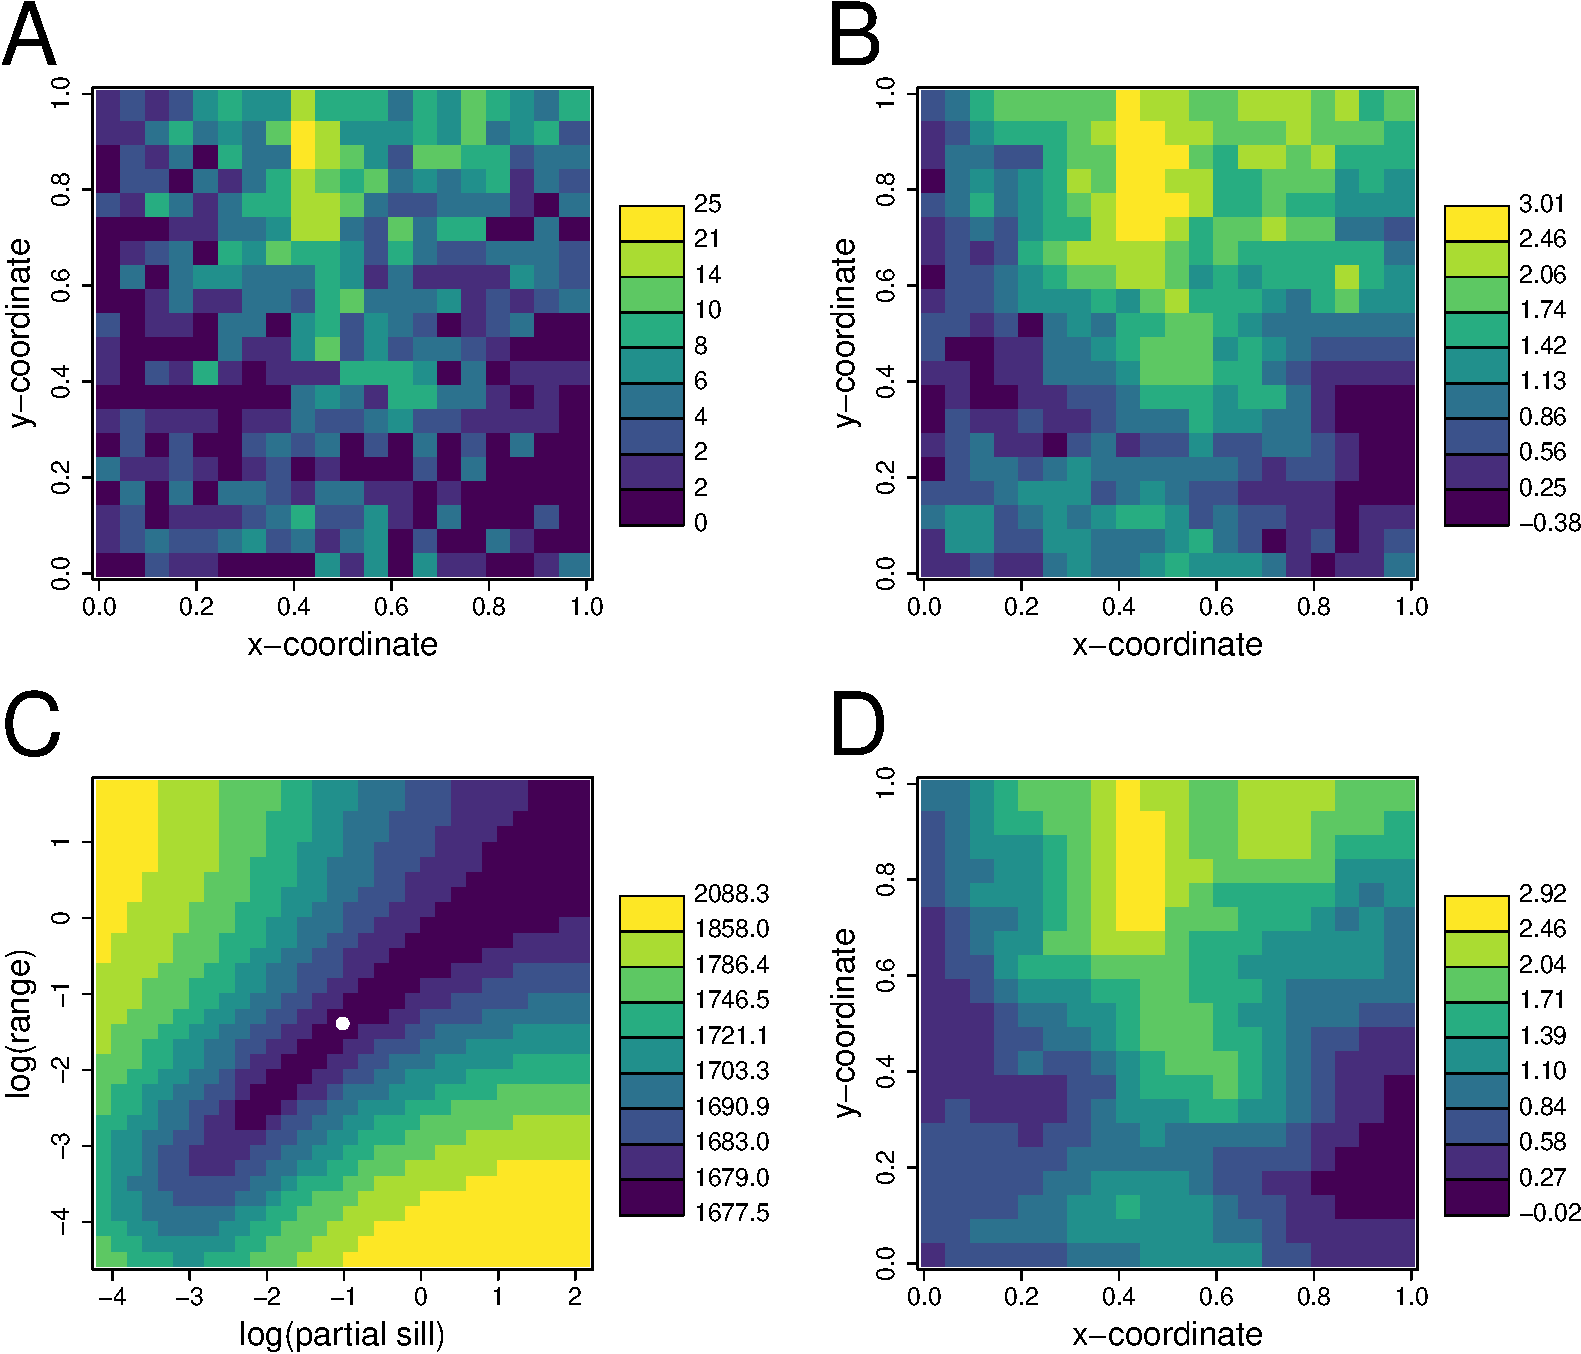
\includegraphics[width=.95\linewidth]{figures/pois_likelihood_estimation}
  \end{center}
  \caption{Estimation for simulated data. A. Simulated count data using the model described in the text.  B. The true simulated $\mathbf{w}$ values. C. The likelihood surface of the simulated data.  The white circle shows the estimated value.  D. The estimated $\hat{\mathbf{w}}$ values. \label{Fig:sglm_likelihood_estimation}}
\end{figure}

%                        Figure TexTurn_scatter
\begin{figure}[H]
  \begin{center}
	    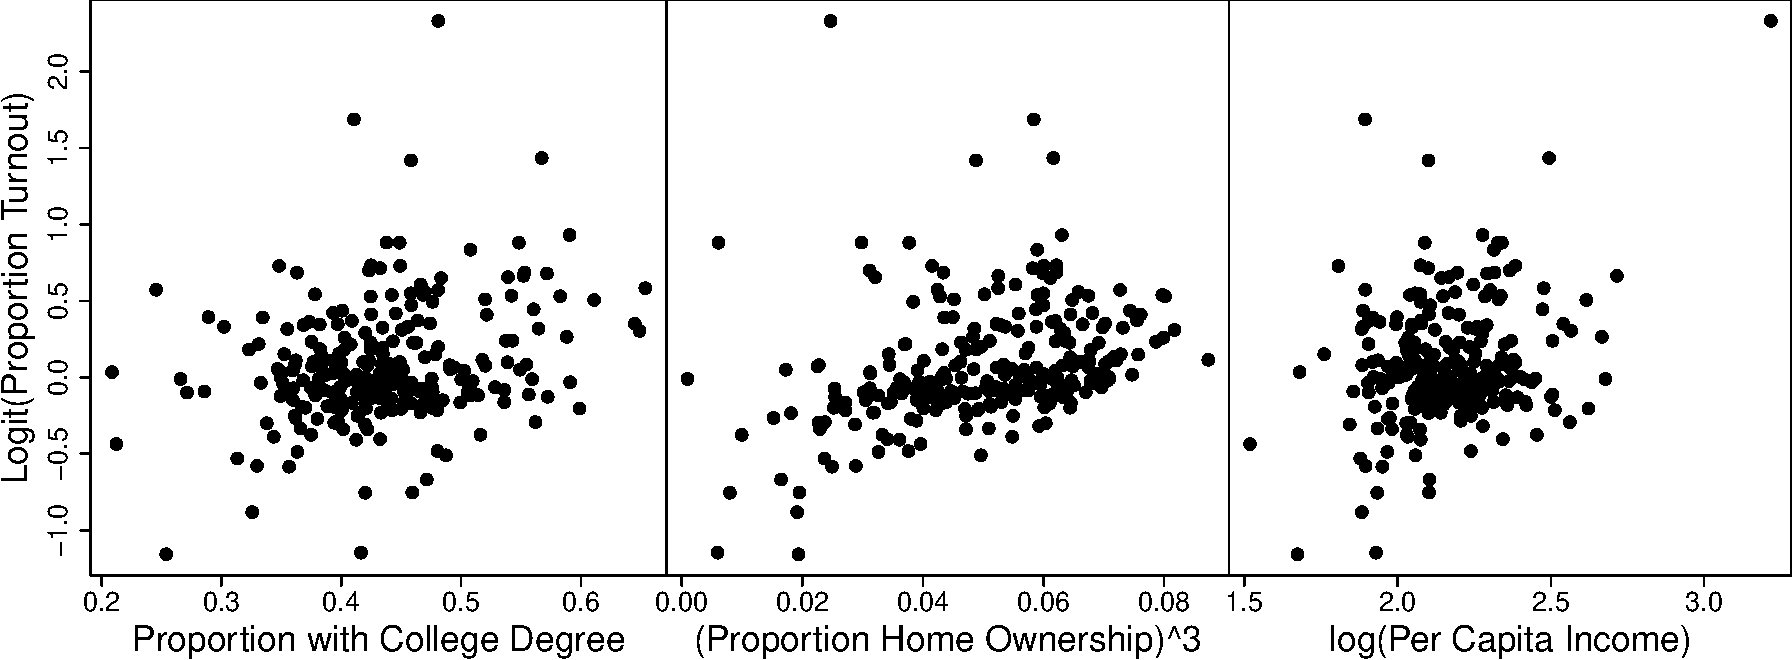
\includegraphics[width=.95\linewidth]{figures/TexTurn_scatter}
  \end{center}
  \caption{Scatterplot of the logit of voter-turnout response variable by the three explanatory variables.  Note the transformations of some explanatory variables, where proportion of home ownership was cubed, and natural logs were taken of per capital income.  \label{Fig:TexTurn_scatter}}
\end{figure}

%                         Figure Texturn_maps
\begin{figure}[H]
  \begin{center}
	    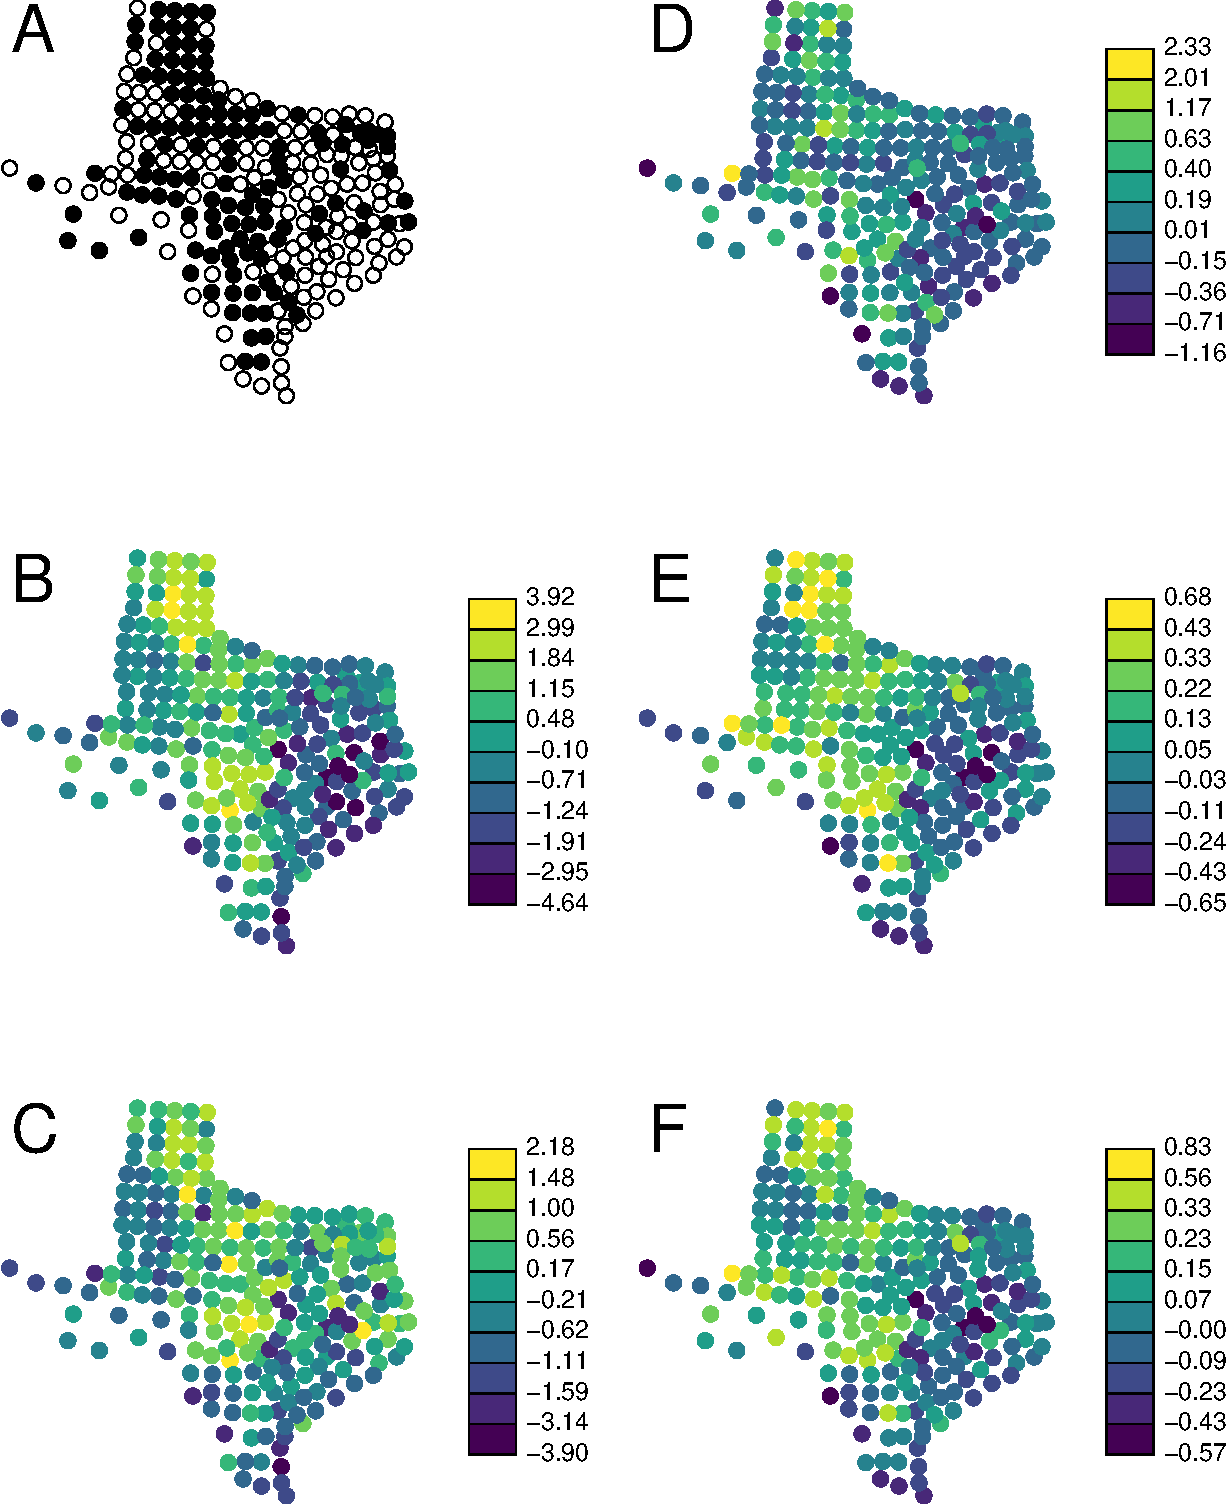
\includegraphics[width=.88\linewidth]{figures/TexTurn_maps}
  \end{center}
  \caption{Raw data and predicted spatial random effects ($\bw$) for the Texas turnout data. A) raw binary data, where open circles are zeros and solid circles are ones, B) predicted $\hat{\bw}$ using SAR model for binary data, C) predicted $\hat{\bw}$ using CAR model for binary data, D) logit-transformed proportional turnout data, E) predicted $\hat{\bw}$ using SAR model for proportional turnout data, F) predicted $\hat{\bw}$ using CAR model for proportional turnout data.\label{Fig:TexTurn_maps}}
\end{figure}

%                         Figure TexTurn_histpdf
\begin{figure}[H]
  \begin{center}
	    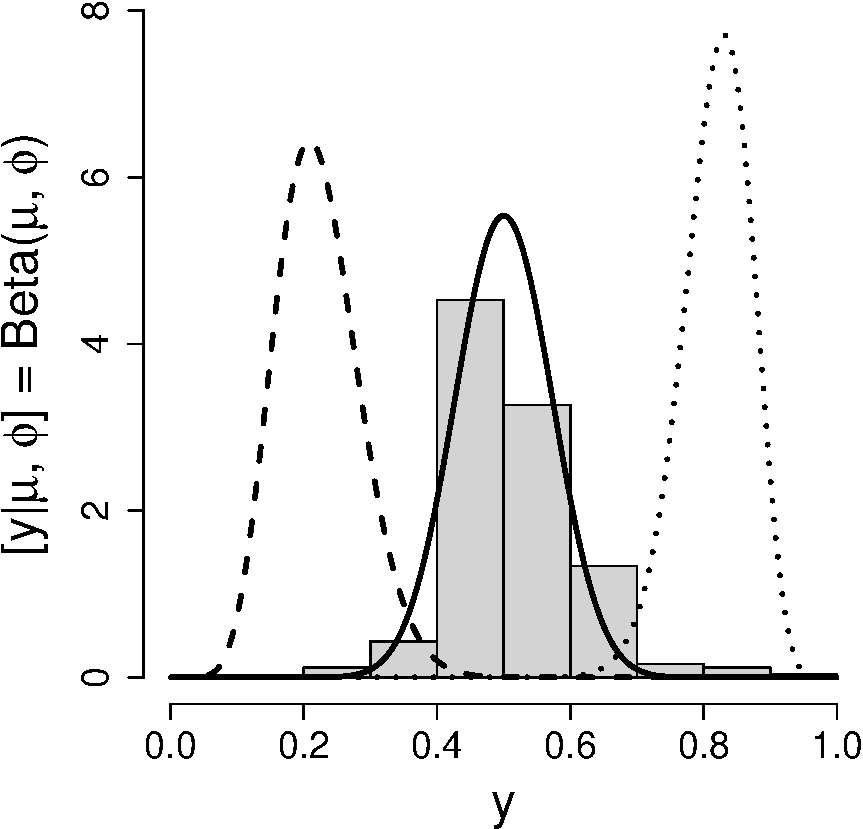
\includegraphics[width=.95\linewidth]{figures/TexTurn_histpdf}
  \end{center}
  \caption{Histogram of proportional turnout and fitted probability density functions for a beta distribution with $\phi = 46.9$ at $\mu$ values of 0.3 (dashed line), 0.5 (solid line), and 0.8 (dotted line). \label{Fig:TexTurn_histpdf}}
\end{figure}

%                         Figure seals_explanvar
\begin{figure}[H]
  \begin{center}
	    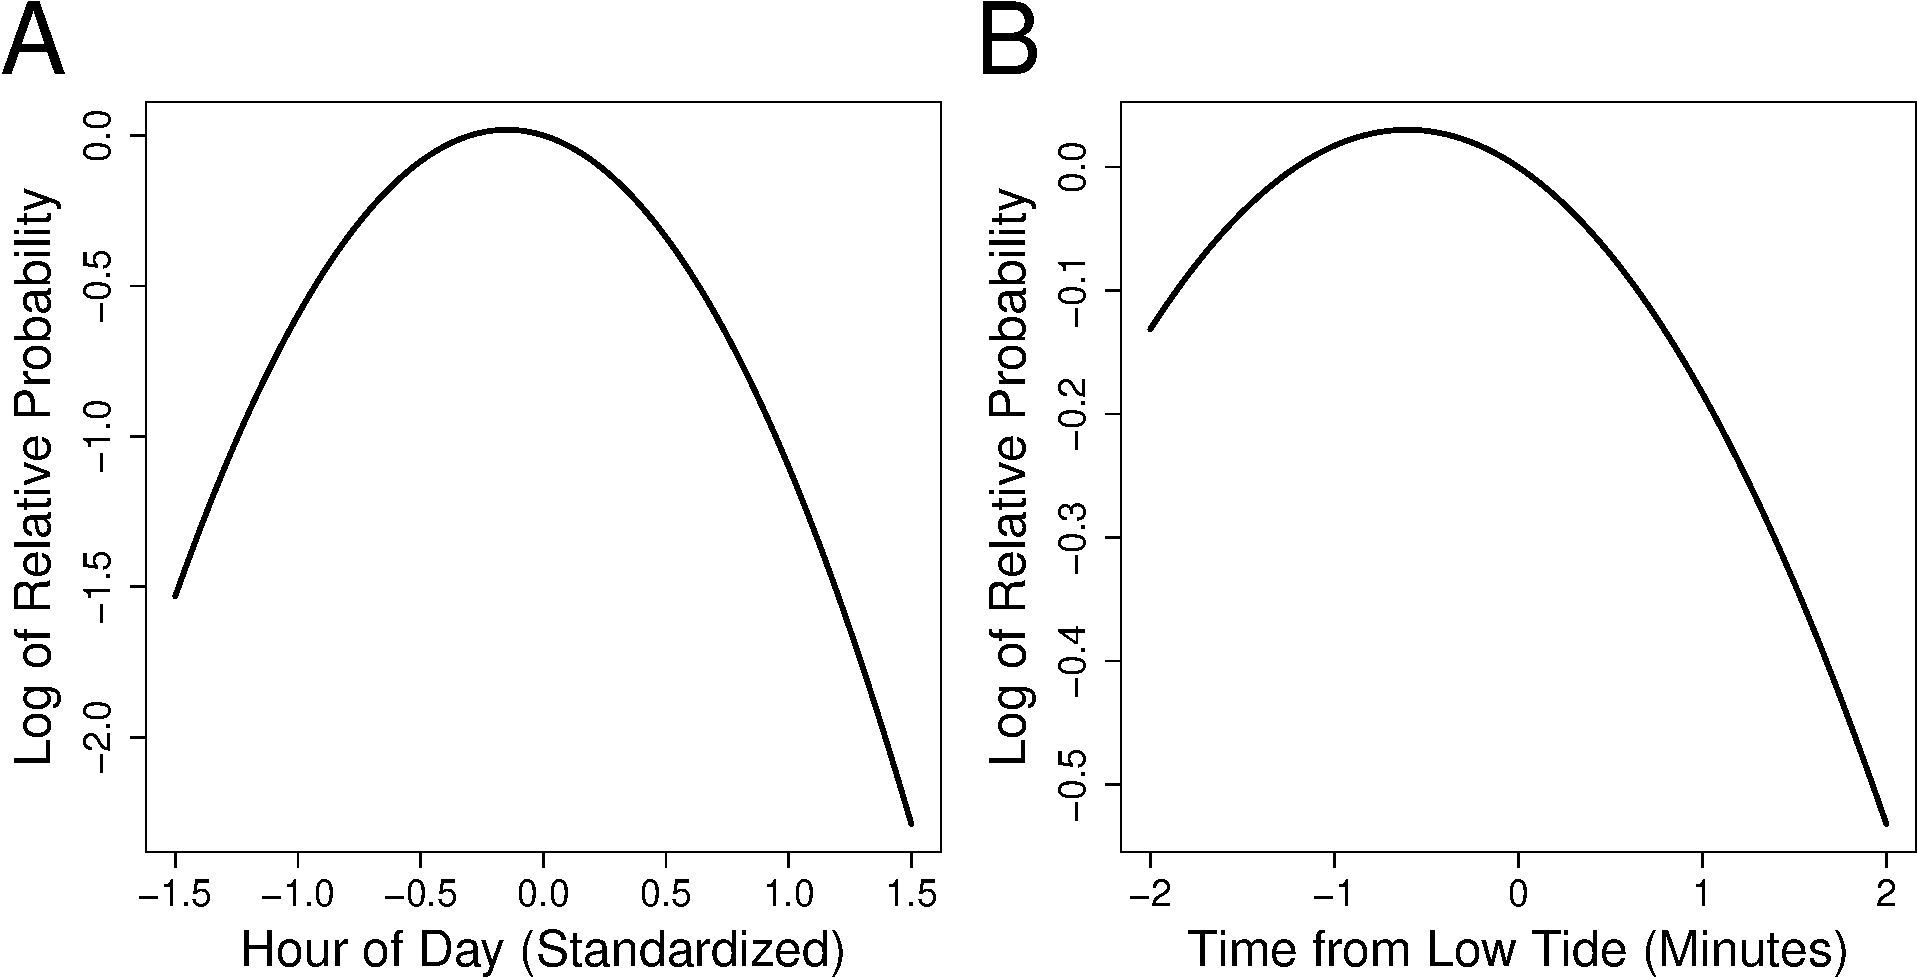
\includegraphics[width=.95\linewidth]{figures/seals_explanvar}
  \end{center}
  \caption{Fitted effects of A) hour-of-day and B) time-from-low-tide on harbor seal counts.  The fitted effect shows the log of the expected proportional change from the zero value of all covariates. \label{Fig:seals_explanvar}}
\end{figure}

%                         Figure seals_predw
\begin{figure}[H]
  \begin{center}
	    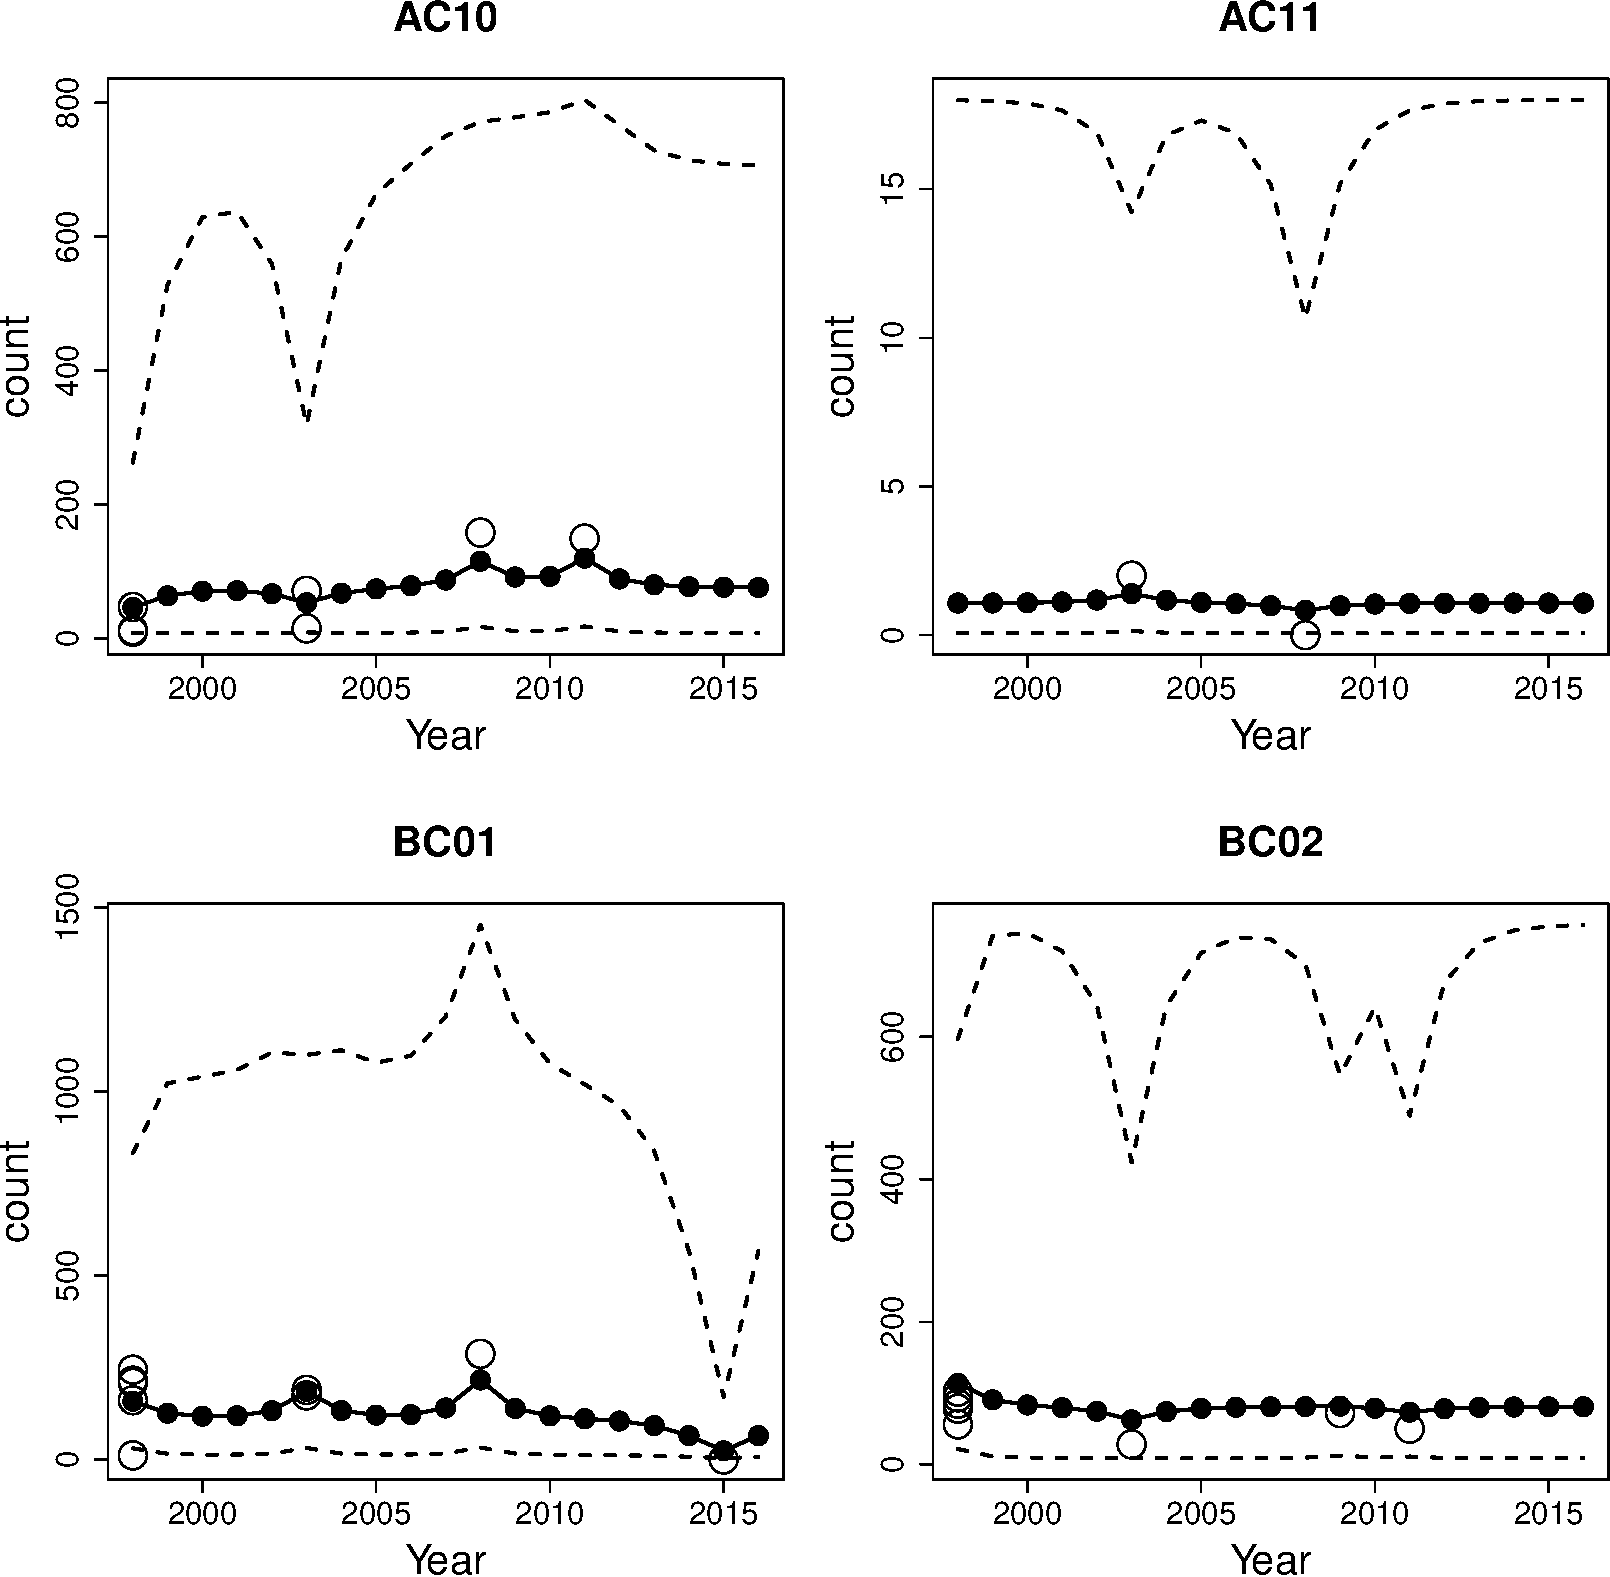
\includegraphics[width=.95\linewidth]{figures/seals_predw}
  \end{center}
  \caption{Predicted $w$-values for 4 of the 74 sites.  Open circles are raw counts, and solid circles are predicted $w$-values connected by a solid line.  The dashed line shows the prediction intervals.  \label{Fig:seals_predw}}
\end{figure}

%                         Figure moss_densities
\begin{figure}[H]
  \begin{center}
	    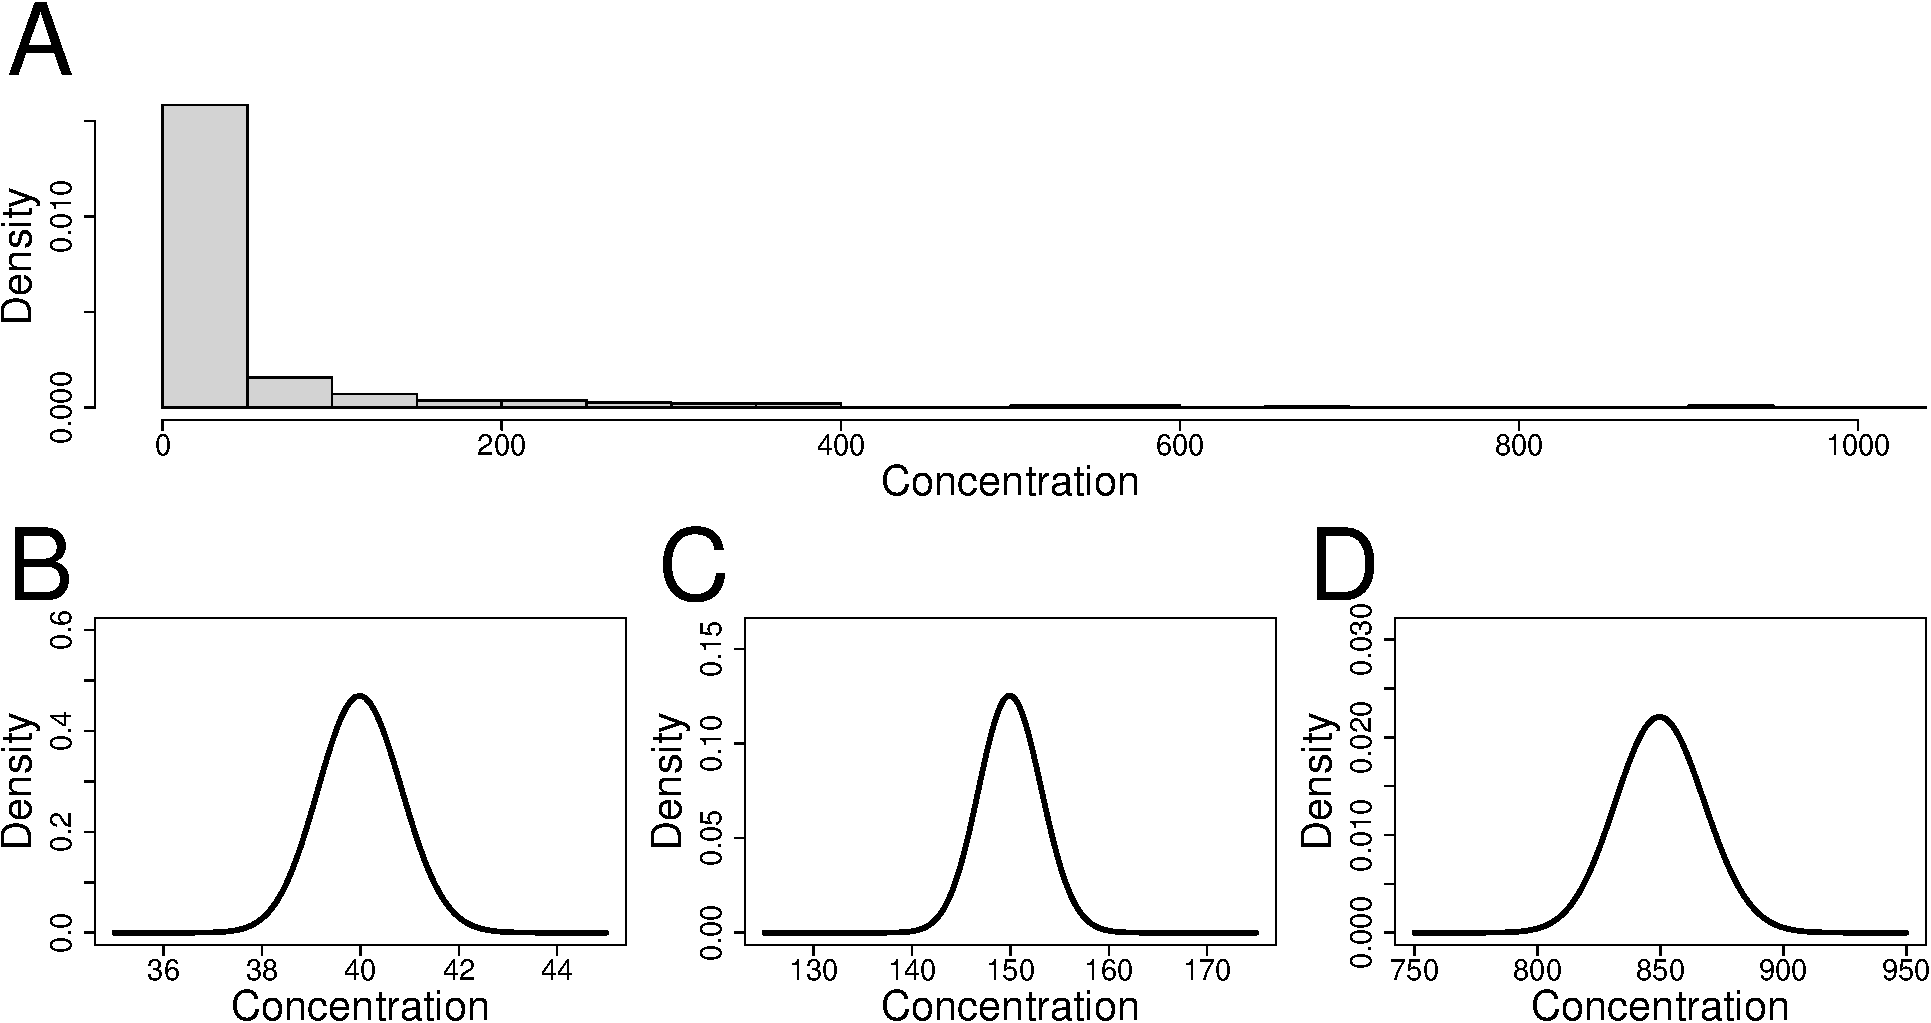
\includegraphics[width=.95\linewidth]{figures/moss_densities}
  \end{center}
  \caption{A) Histogram of lead concentration in moss, B) fitted probability density at $\mu = 40$ with $\phi = 2218$ for the gamma distribution (solid line) C) $\mu = 150$, and D) $\mu = 850$. \label{Fig:moss_densities}}
\end{figure}

%                           Figure moss_maps
\begin{figure}[H]
  \begin{center}
	    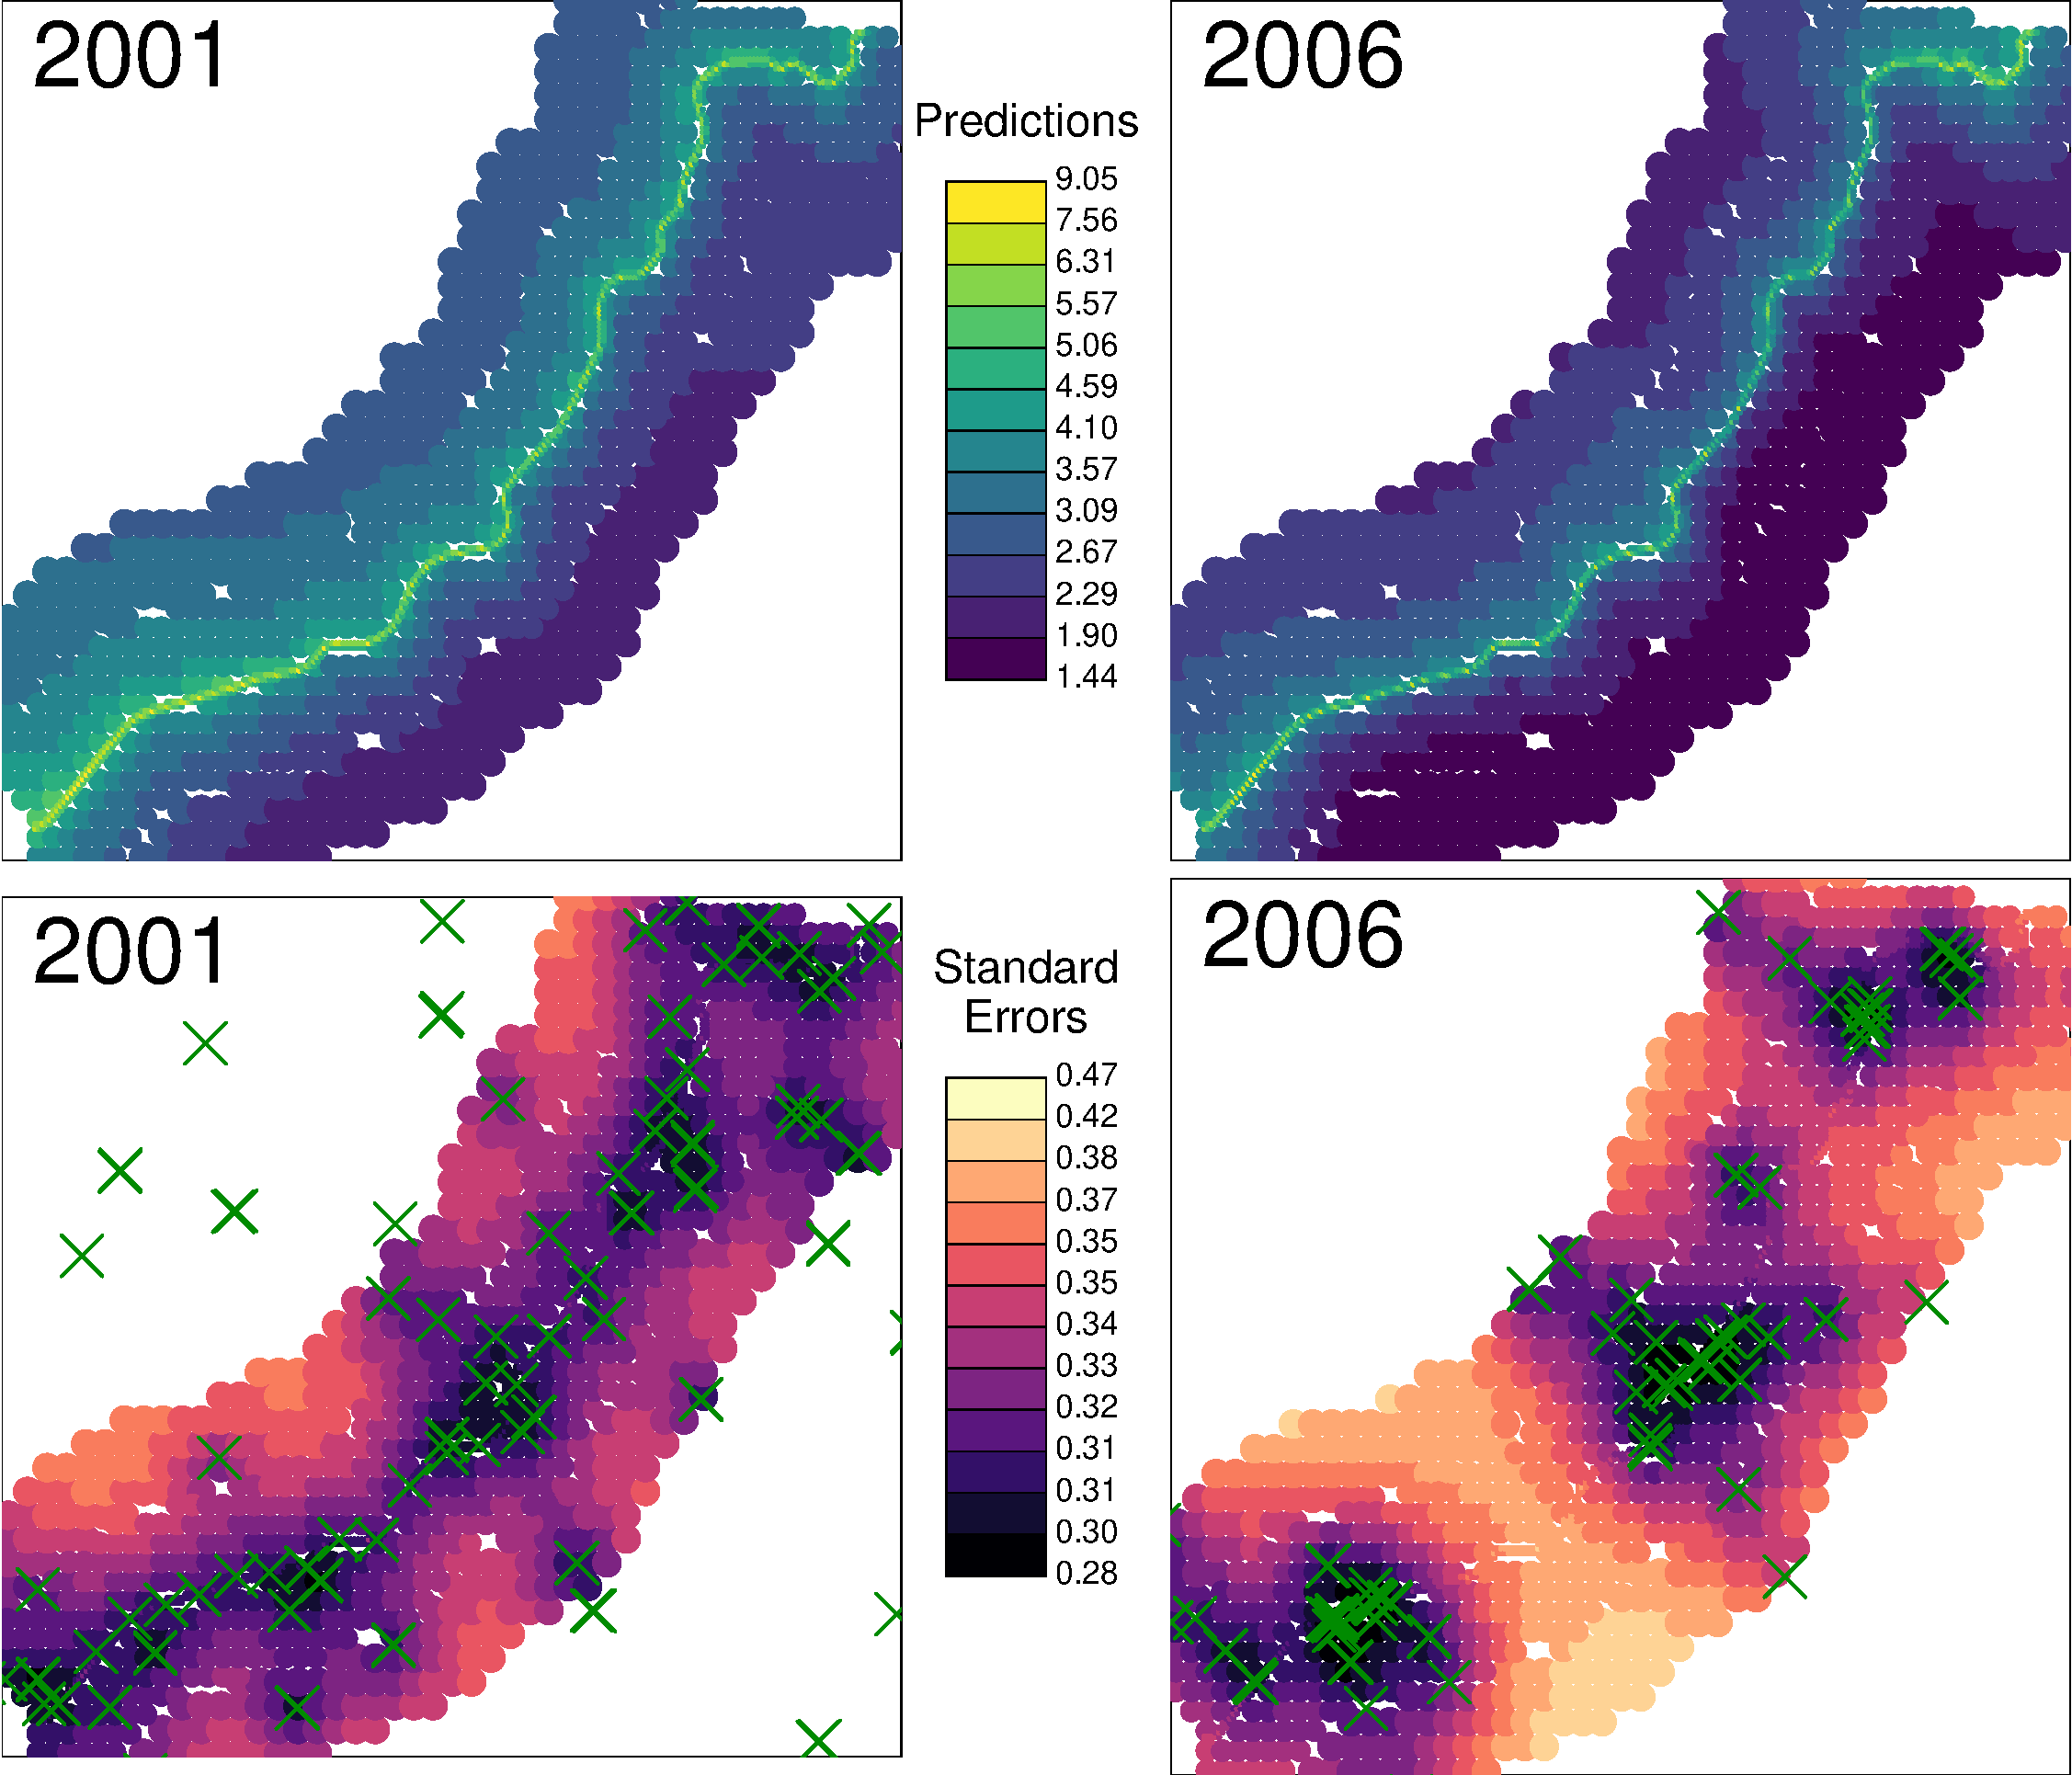
\includegraphics[width=.95\linewidth]{figures/moss_maps}
  \end{center}
  \caption{Prediction and their standard errors for 2001 and 2006 at locations near the haul road through Cape Krusenstern National Park, Alaska.  The green $\times$ symbols show sample locations. \label{Fig:moss_maps}}
\end{figure}


%%%%%%%%%%%%%%%%%%%%%%%%%%%%%%%%%%%%%%%%%%%%%%%%%%%%%%%%%%%%%%%%%%%%%%%%%%%%%%%%%%
%%%%%%%%%%%%%%%%%%%%%%%%%%%%%%%%%%%%%%%%%%%%%%%%%%%%%%%%%%%%%%%%%%%%%%%%%%%%%%%%%%
%              APPENDIX
%%%%%%%%%%%%%%%%%%%%%%%%%%%%%%%%%%%%%%%%%%%%%%%%%%%%%%%%%%%%%%%%%%%%%%%%%%%%%%%%%%
%%%%%%%%%%%%%%%%%%%%%%%%%%%%%%%%%%%%%%%%%%%%%%%%%%%%%%%%%%%%%%%%%%%%%%%%%%%%%%%%%%


\clearpage
\setcounter{equation}{0}
\renewcommand{\theequation}{A.\arabic{equation}}
\setcounter{figure}{0}
\renewcommand{\thefigure}{A.\arabic{figure}}
\section{APPENDIX}

%------------------------------------------------------------------------------
% Appendix A: Derivation REML from Integration
%------------------------------------------------------------------------------

\subsection{Derivation of REML from Integration}
\noindent
Consider a multivariate normal distribution for a general linear model,
\begin{equation} \label{eq:MVNdist}
[\mathbf{y};\bbeta,\btheta] = 
\frac{\exp\left(-\frac{1}{2}(\mathbf{y} - \mathbf{X}\bbeta)\upp\bSigma^{-1}(\mathbf{y} - \mathbf{X}\bbeta)\right)}{(2\pi)^{n/2}|\bSigma|^{1/2}},
\end{equation}
where $\mathbf{y}$ is an $n \times 1$ vector for the response variable, $\mathbf{X}$ is a $n \times p$ design matrix of explanatory variables, $\bbeta$ is a $p \times 1$ vector of fixed effects, $\btheta$ contains covariance parameters contained in the $n \times n$ covariance matrix $\bSigma$. It is possible to obtain REML equations by integrating out the fixed effects $\bbeta$,
$$
\int_{\mathbb{R}^p} f(\mathbf{y};\bbeta,\btheta) d\bbeta,
$$
to obtain a likelihood that is a function of just the covariance parameters $\btheta$ and the data $\mathbf{y}$.  In particular
$$
-2 \ln \left(\int_{\mathbb{R}^p} f(\mathbf{y};\bbeta,\btheta) d\bbeta \right) = (n - p)\ln(2\pi) + \ln|\bSigma| + \ln|\mathbf{X}\upp\bSigma^{-1}\mathbf{X}| + (\mathbf{y} - \mathbf{X}\hat{\bbeta})\upp\bSigma^{-1}(\mathbf{y} - \mathbf{X}\hat{\bbeta}),
$$
where $\hat{\bbeta} = (\mathbf{X}\upp\bSigma^{-1}\mathbf{X})^{-1}\mathbf{X}\upp\bSigma^{-1}\mathbf{y}$. \\

{\large \flushleft \textbf{Proof}}

\flushleft Write \eqref{eq:MVNdist} as
\begin{align*}
[\mathbf{y};\bbeta,\btheta] & = 
\frac{\exp\left(-\frac{1}{2}(\mathbf{y} - \mathbf{X}\hat{\bbeta} + \mathbf{X}\hat{\bbeta} - \mathbf{X}\bbeta)\upp\bSigma^{-1}(\mathbf{y} - \mathbf{X}\hat{\bbeta} + \mathbf{X}\hat{\bbeta} -  \mathbf{X}\bbeta)\right)}{(2\pi)^{n/2}|\bSigma|^{1/2}}, \\
{} & = 
\frac{\exp\left(-\frac{1}{2}[(\mathbf{y} - \mathbf{X}\hat{\bbeta})\bSigma^{-1}(\mathbf{y} - \mathbf{X}\hat{\bbeta}) + (\mathbf{X}\hat{\bbeta} - \mathbf{X}\bbeta)\upp\bSigma^{-1}(\mathbf{X}\hat{\bbeta} -  \mathbf{X}\bbeta) + C\right)}{(2\pi)^{n/2}|\bSigma|^{1/2}},
\end{align*}
where $C = 2(\mathbf{y} - \mathbf{X}\hat{\bbeta})\upp\bSigma^{-1}(\mathbf{X}\hat{\bbeta} - \mathbf{X}\bbeta)$ = 0.
Factor out terms that do not contain $\bbeta$,
$$
\int_{\mathbb{R}^p} [\mathbf{y};\bbeta,\btheta] d\bbeta = M
\int_{\mathbb{R}^p} \exp\left(-\frac{1}{2}(\mathbf{X}\hat{\bbeta} - \mathbf{X}\bbeta)\upp\bSigma^{-1}(\mathbf{X}\hat{\bbeta} -  \mathbf{X}\bbeta)\right)d\bbeta,
$$
where $M = \exp[-\frac{1}{2}(\mathbf{y} - \mathbf{X}\hat{\bbeta})\bSigma^{-1}(\mathbf{y} - \mathbf{X}\hat{\bbeta})]/[(2\pi)^{n/2}|\bSigma|^{1/2}]$.
Notice that
\begin{align*}
	{} & \int_{\mathbb{R}^p} \exp\left(-\frac{1}{2}(\mathbf{X}\hat{\bbeta} - \mathbf{X}\bbeta)\upp\bSigma^{-1}(\mathbf{X}\hat{\bbeta} -  \mathbf{X}\bbeta)\right)d\bbeta, \\
  = & \int_{\mathbb{R}^p} \exp\left(-\frac{1}{2}(\bbeta - \hat{\bbeta})\upp(\mathbf{X}\upp\bSigma^{-1}\mathbf{X})(\bbeta -  \hat{\bbeta})\right)d\bbeta, \\
	= & 2\pi^{p/2}|(\mathbf{X}\upp\bSigma^{-1}\mathbf{X})|^{-1/2},
\end{align*}
by recalling that, for positive definite $\bA_{m \times m}$ and any conformable $\bx \ne \bzero$,
$$
	\int_{\mathbb{R}^m}\exp(-\mathbf{x}\upp\mathbf{A}\mathbf{x}/2) d\mathbf{x} = (2\pi)^{m/2}|\mathbf{A}|^{-1/2}.
$$
Hence, we arrive at
$$
[\mathbf{y};\btheta] = \int_{\mathbb{R}^p} [\mathbf{y};\bbeta,\btheta] d\bbeta = \frac{\exp\left(-\frac{1}{2}(\mathbf{y} - \mathbf{X}\hat{\bbeta})\upp\bSigma^{-1}(\mathbf{y} - \mathbf{X}\hat{\bbeta})\right)}{(2\pi)^{(n-p)/2}|\bSigma|^{1/2}|\mathbf{X}\upp\bSigma^{-1}\mathbf{X}|^{1/2}},
$$
and taking $-2 \ln [\mathbf{y};\btheta]$ we obtain the desired result.

%------------------------------------------------------------------------------
% Appendix B: Inverse Gaussian Distribution
%------------------------------------------------------------------------------

\clearpage
\subsection{Distribution Parameterizations}

\subsubsection{Negative Binomial Distribution}

\noindent{} For the negative binomial, $y_{i}$ is a non-negative integer with probability density function (PDF)
$$
[y|\mu,\phi] = 
\frac{\Gamma(y + \phi)}{\Gamma(\phi)y!}
\left(
\frac{\mu}{\mu + \phi}
\right)^{y}
\left(
\frac{\phi}{\mu + \phi}
\right)^{\phi},
$$
where $0 < \mu < 1$, $0 < \phi$, $\textrm{E}(Y) = \mu$, $\var(Y) = \mu + \mu^{2}/\phi$, and $\Gamma(\cdot)$ is the gamma function.

\subsubsection{Gamma Distribution}

\noindent{} For the gamma distribution, $y_{i}$ is positive with PDF
$$
[y|\mu,\phi] = \frac{1}{\Gamma(\phi)} \left(\frac{\phi}{\mu}\right)^\phi y^{\phi - 1}\exp\left(\frac{-y\phi}{\mu}\right),
$$
where $0 < \mu$, $0 < \phi$, , $\textrm{E}(Y) = \mu$, and $\var(Y) = \mu^{2}/\phi$.{}

\subsubsection{Beta Distribution}

\noindent{} For the beta distribution, $0 < y_{i} < 1$ with PDF
$$
[y|\mu,\phi] = \frac{\Gamma(\phi)}{\Gamma(\mu\phi)\Gamma((1-\mu)\phi)}y^{\mu\phi - 1}(1 - y)^{(1-\mu)\phi - 1},
$$
where $0 < \mu < 1$, $0 < \phi$, $\textrm{E}(Y) = \mu$, and $\var(Y) = \mu(1 - \mu)/(1 + \phi)$. 

\subsubsection{Inverse Gaussian Distribution}

\noindent{} The inverse Gaussian distribution is usually written as,
\begin{equation} \label{eq:IGdist}
[y;\mu,\lambda] = 
\sqrt{\frac{\lambda}{2\pi y^{3}}}\exp\left(-\frac{\lambda(y - \mu)^{2}}{2\mu^{2} y}\right),
\end{equation}
where $y > 0$, $\mu > 0$, and $\lambda > 0$. In this parameterization $\lambda$ is a shape parameter, and $\textrm{E}(Y) = \mu$ and $\var(Y) = \mu^{3}/\lambda$.  In order to keep $\mu$ positive and $w$ unconstrained in \eqref{eq:lm_eta}, we let $\bmu = \exp(\bw)$.  However, under this construction, from \eqref{eq:Dii}, we obtain
$$
D_{i,i} = \frac{(e^{w_{i}} - 2 y_{i})}{\phi e^{2 w_{i}} },
$$
and some $D_{i,i}$ can be positive whenever $e^{w_{i}} > 2y_{i}$, which can lead to $\bH$ in \eqref{eq:Hdef} being singular.  We propose an alternative parameterization.  For inverse Gaussian models, $\lambda$ is often scaled, and here we do so by taking $\phi = \lambda/\mu = \lambda/\exp(w)$, yielding a $\mu$-scaled-$\lambda$ inverse Gaussian model,
\begin{equation} \label{eq:phiIGdist}
[y;\mu,\lambda] = 
\sqrt{\frac{\phi\exp(w)}{2\pi y^{3}}}\exp\left(-\frac{\phi(y - \exp(w))^{2}}{2\exp(w) y}\right),
\end{equation}
where $\phi > 0$ and now $\var(Y) = \mu^{2}/\phi$.  Under this parameterization, we have
%second derivative of log(exp(w)*phi/(2*pi*y^3))/2-phi*(y - exp(w))^2/(2y*exp(w)) with respect to w
$$
D_{i,i} = -\frac{\phi(e^{2w_{i}} + y_{i}^{2})}{2 y e^{w_{i}} },
$$
which is always negative, and so \eqref{eq:Hdef} is always well-behaved.  Under this construction, we also have
$$
d_{i} = \phi\left(\frac{y}{2e^{w_{i}}} - \frac{ e^{w_{i}}}{2y}\right) + \frac{1}{2}.
$$


%%%%%%%%%%%%%%%%%%%%%%%%%%%%%%%%%%%%%%%%%%%%%%%%%%%%%%%%%%%%%%%%%%%%%%%%%%%%%%%%
%%%%%%%%%%%%%%%%%%%%%%%%%%%%%%%%%%%%%%%%%%%%%%%%%%%%%%%%%%%%%%%%%%%%%%%%%%%%%%%%
%%%%%%%%%%%            %%%%%%%    %%%%%%%%  %%%%%%%       %%%%%%%%%%%%%%%%%%%%%%
%%%%%%%%%%%  %%%%%%%%%%%%%%%%%  %  %%%%%%%  %%%%%%%  %%%%  %%%%%%%%%%%%%%%%%%%%%
%%%%%%%%%%%  %%%%%%%%%%%%%%%%%  %%  %%%%%%  %%%%%%%  %%%%%%  %%%%%%%%%%%%%%%%%%%
%%%%%%%%%%%  %%%%%%%%%%%%%%%%%  %%%  %%%%%  %%%%%%%  %%%%%%%   %%%%%%%%%%%%%%%%%
%%%%%%%%%%%            %%%%%%%  %%%%  %%%%  %%%%%%%  %%%%%%%%  %%%%%%%%%%%%%%%%%
%%%%%%%%%%%  %%%%%%%%%%%%%%%%%  %%%%%  %%%  %%%%%%%  %%%%%%%   %%%%%%%%%%%%%%%%%
%%%%%%%%%%%  %%%%%%%%%%%%%%%%%  %%%%%%  %%  %%%%%%%  %%%%%%  %%%%%%%%%%%%%%%%%%%
%%%%%%%%%%%  %%%%%%%%%%%%%%%%%  %%%%%%%  %  %%%%%%%  %%%%  %%%%%%%%%%%%%%%%%%%%%
%%%%%%%%%%%            %%%%%%%  %%%%%%%%    %%%%%%%       %%%%%%%%%%%%%%%%%%%%%%
%%%%%%%%%%%%%%%%%%%%%%%%%%%%%%%%%%%%%%%%%%%%%%%%%%%%%%%%%%%%%%%%%%%%%%%%%%%%%%%%
%%%%%%%%%%%%%%%%%%%%%%%%%%%%%%%%%%%%%%%%%%%%%%%%%%%%%%%%%%%%%%%%%%%%%%%%%%%%%%%%


\end{document}

